%!TEX root = origin.TEX
\chapter{Desarrollo de la Investigación}
\pagenumbering{arabic}
\setcounter{page}{82}
\renewcommand{\baselinestretch}{1.2} %doble espacio paratodo el texto

En la siguiente imagen se detallan los procesos de implementación computacional más importantes que fueron realizados durante el desarrollo de la investigación:

\begin{figure}[H]
	\begin{center}
	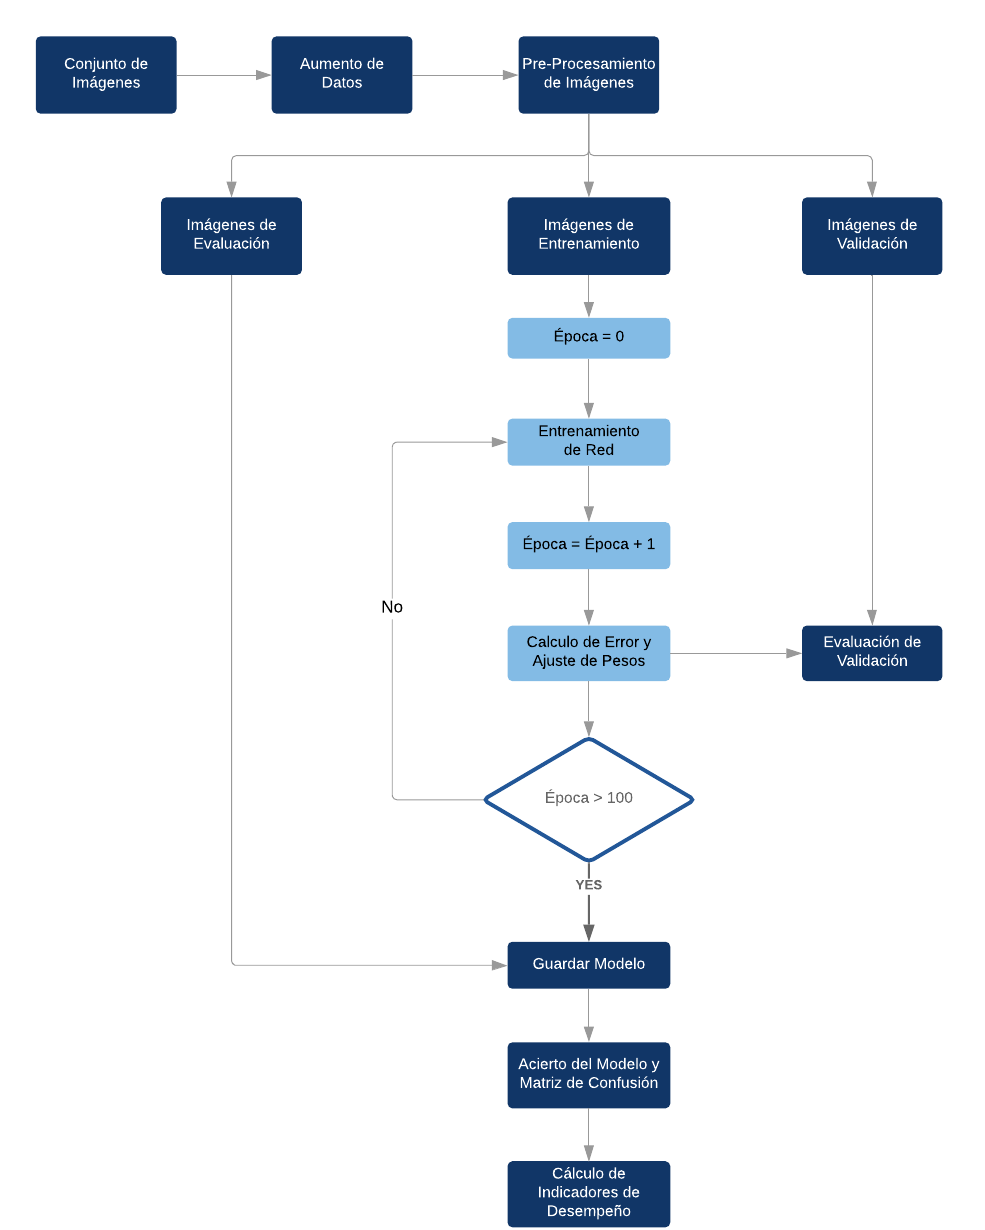
\includegraphics[width=1\textwidth,height=17cm]{images/summaryflowchart}
	\end{center}
	\vspace{1.5em}
	\begin{center}
	\caption{\small{Diagrama de flujo para el desarrollo de la Investigación}}
	\vskip -0.25cm
	{\small{Fuente: Elaboración propia}}
	\end{center}
	
\end{figure}


\section{Análisis del conjunto de Imágenes}
	
	En esta etapa de la investigación se busca encontrar imágenes de señales de tránsito, las cuales conforman la principal fuente de los modelos que se pretenden crear. Estas será usadas durante el entrenamiento, validación y evaluación del modelo pretendido.
	
	\subsection{Datos Iniciales para el entrenamiento}
		Se obtienen un conjunto de imágenes iniciales de señales de tránsito de Alemania y Perú, las cuales servirán para entrenar y validar los modelos creados.
		\subsubsection{Señales de Tránsito de Alemania}

			En esta colección consta de un total de 51839 imágenes distribuidas en 43 clases no necesariamente balanceadas con un tamaño de 32 x 32 pixeles.

			\begin{figure}[H]
				\begin{center}
				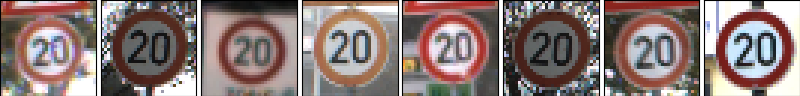
\includegraphics[width=1\textwidth]{images/desarrollo/imagenes/alemania/1__(1).png}
				\end{center}
				\begin{center}
				\caption{\small{Speed limit (20km/h)}}
				\vskip -0.25cm
				{\small{Fuente: Elaboración propia}}
				\end{center}
				\vspace{-1.5em}
			\end{figure}

			%\begin{figure}[H]
				%\begin{center}
				%
\includegraphics[width=1\textwidth]{images/desarrollo/imagenes/alemania/1__(2).png}
				%\end{center}
				%\begin{center}
				%\caption{\small{Speed limit (30km/h)}}
				%\end{center}
				%\vspace{-1.5em}
			%\end{figure}

			\begin{figure}[H]
				\begin{center}
				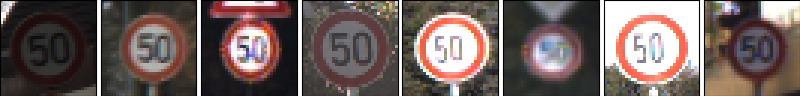
\includegraphics[width=1\textwidth]{images/desarrollo/imagenes/alemania/1__(3).png}
				\end{center}
				\begin{center}
				\caption{\small{Speed limit (50km/h)}}
				\vskip -0.25cm
				{\small{Fuente: Elaboración propia}}
				\end{center}
				\vspace{-1.5em}
			\end{figure}

			%\begin{figure}[H]
				%\begin{center}
				%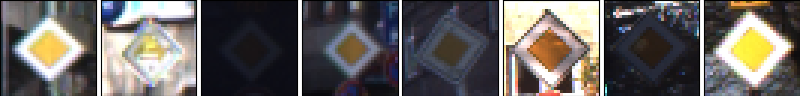
\includegraphics[width=1\textwidth]{images/desarrollo/imagenes/alemania/1__(13).png}
				%\end{center}
				%\begin{center}
				%\caption{\small{Priority road}}
				%\end{center}
				%\vspace{-1.5em}
			%\end{figure}
			
			\begin{figure}[H]
				\begin{center}
				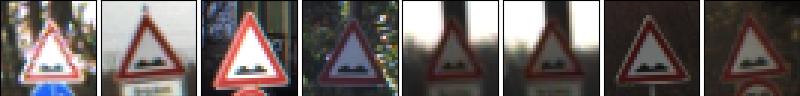
\includegraphics[width=1\textwidth]{images/desarrollo/imagenes/alemania/1__(23).png}
				\end{center}
				\begin{center}
				\caption{\small{Bumpy road}}
				\vskip -0.25cm
				{\small{Fuente: Elaboración propia}}
				\end{center}
				\vspace{-1.5em}
			\end{figure}

			\begin{figure}[H]
				\begin{center}
				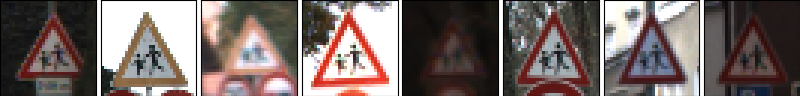
\includegraphics[width=1\textwidth]{images/desarrollo/imagenes/alemania/1__(29).png}
				\end{center}
				\begin{center}
				\vskip -0.25cm
				{\small{Fuente: Elaboración propia}}
				\caption{\small{Children crossing}}
				\end{center}
				\vspace{-1.5em}
			\end{figure}
			

			\begin{figure}[H]
				\begin{center}
				
\includegraphics[width=1\textwidth]{images/desarrollo/imagenes/alemania/1__(35).png}
				\end{center}
				\begin{center}
				\caption{\small{Turn left ahead}}
				\vskip -0.25cm
				{\small{Fuente: Elaboración propia}}
				\end{center}
				\vspace{-1.5em}
			\end{figure}

			\vskip 0.75cm
			\begin{figure}[H]
				\begin{center}
				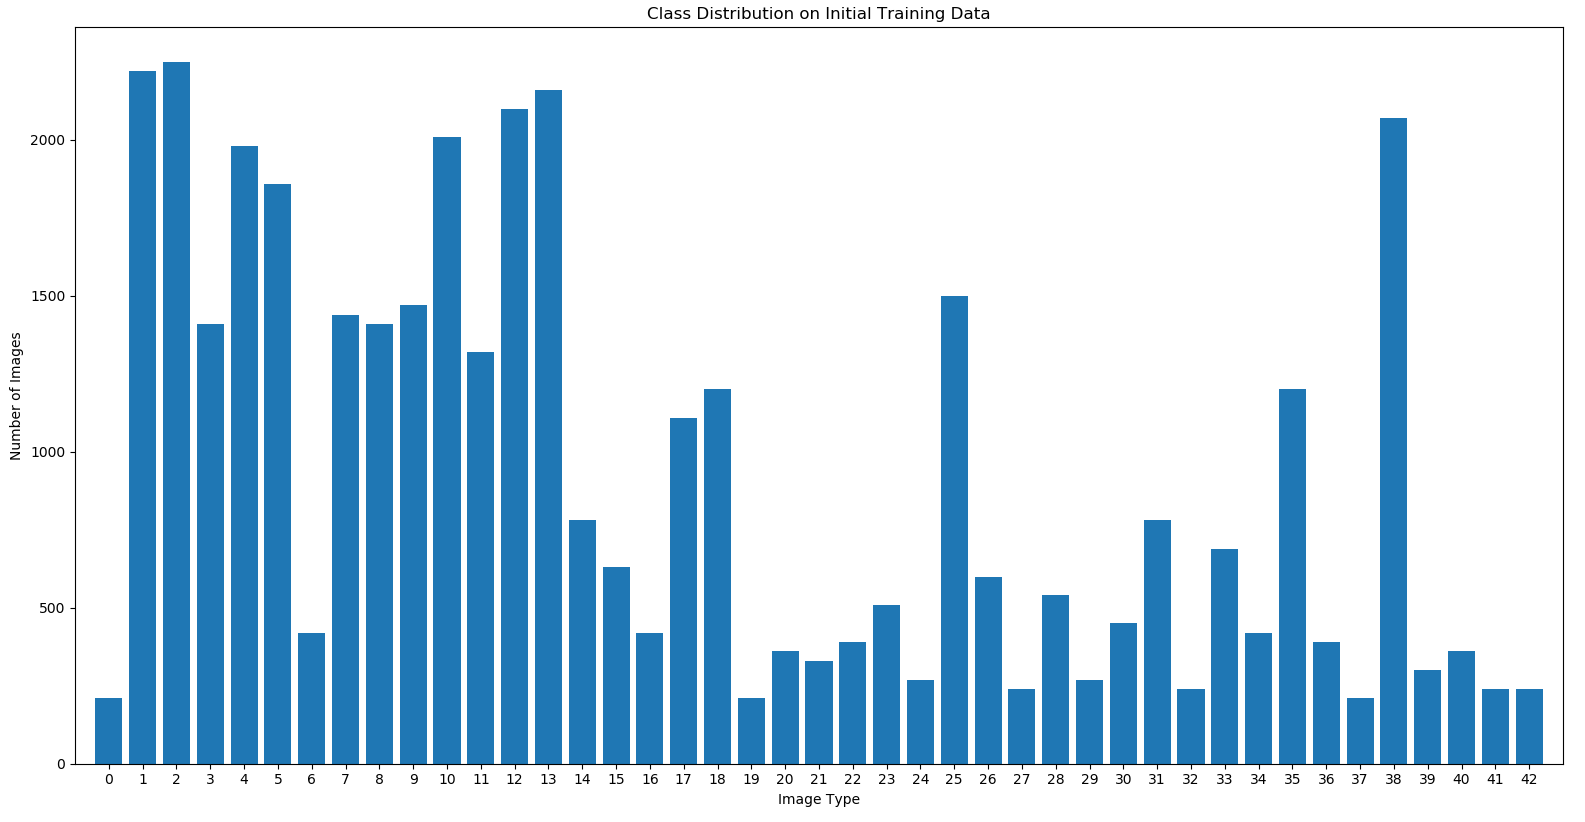
\includegraphics[width=1\textwidth, height=1.2\textheight,keepaspectratio]{images/desarrollo/histograms/initial39209}
				\end{center}
				\begin{center}
				\caption{\small{Distribución de ejemplos por señal para el entrenamiento(Total 39209)}}	
				{\small{\fontsize{10}{16.8}\selectfont {Fuente: Elaboración propia}}}
				\end{center}
				\vspace{-1.5em}
			\end{figure}


		\subsubsection{Señales de Tránsito de Perú}

			En esta colección consta de un total de 614 imágenes distribuidas en 7 clases no necesariamente balanceadas con un tamaño de 60 x 60 pixeles.

			\begin{figure}[H]
				\begin{center}
				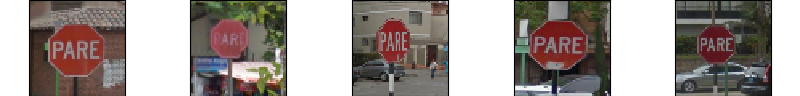
\includegraphics[width=1\textwidth]{images/desarrollo/imagenes/peru/1__(1).png}
				\end{center}
				\begin{center}
				\caption{\small{Pare}}
				\vskip -0.25cm
				{\small{Fuente: Elaboración propia}}
				\end{center}
				\vspace{-1.5em}
			\end{figure}

			\begin{figure}[H]
				\begin{center}
				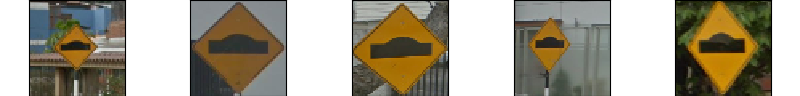
\includegraphics[width=1\textwidth]{images/desarrollo/imagenes/peru/1__(2).png}
				\end{center}
				\begin{center}
				\caption{\small{Resalto}}
				\vskip -0.25cm
				{\small{Fuente: Elaboración propia}}
				\end{center}
				\vspace{-1.5em}
			\end{figure}

			\begin{figure}[H]
				\begin{center}
				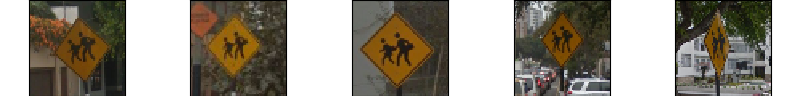
\includegraphics[width=1\textwidth]{images/desarrollo/imagenes/peru/1__(3).png}
				\end{center}
				\begin{center}
				\caption{\small{Zona Escolar}}
				\vskip -0.25cm
				{\small{Fuente: Elaboración propia}}
				\end{center}
				\vspace{-1.5em}
			\end{figure}

			\begin{figure}[H]
				\begin{center}
				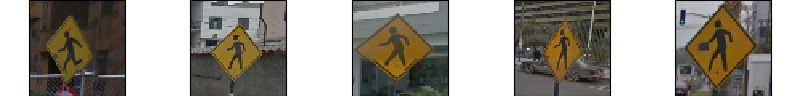
\includegraphics[width=1\textwidth]{images/desarrollo/imagenes/peru/1__(4).png}
				\end{center}
				\begin{center}
				\caption{\small{Peatones}}
				\vskip -0.25cm
				{\small{Fuente: Elaboración propia}}
				\end{center}
				\vspace{-1.5em}
			\end{figure}
			
			\begin{figure}[H]
				\begin{center}
				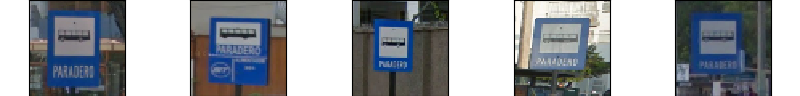
\includegraphics[width=1\textwidth]{images/desarrollo/imagenes/peru/1__(5).png}
				\end{center}
				\begin{center}
				\caption{\small{Paradero}}
				\vskip -0.25cm
				{\small{Fuente: Elaboración propia}}
				\end{center}
				\vspace{-1.5em}
			\end{figure}

			\begin{figure}[H]
				\begin{center}
				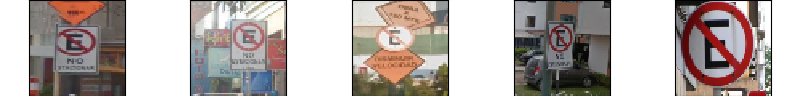
\includegraphics[width=1\textwidth]{images/desarrollo/imagenes/peru/1__(6).png}
				\end{center}
				\begin{center}
				\caption{\small{No Estacionar}}
				\vskip -0.25cm
				{\small{Fuente: Elaboración propia}}
				\end{center}
				\vspace{-1.5em}
			\end{figure}
			
			\begin{figure}[H]
				\begin{center}
				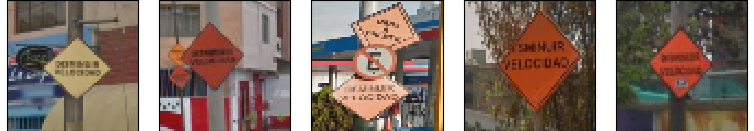
\includegraphics[width=1\textwidth]{images/desarrollo/imagenes/peru/1__(7).png}
				\end{center}
				\begin{center}
				\caption{\small{Disminuir Velocidad}}
				\vskip -0.25cm
				{\small{Fuente: Elaboración propia}}
				\end{center}
				\vspace{-1.5em}
			\end{figure}
			\vskip 2cm
			\begin{figure}[H]
				\begin{center}
				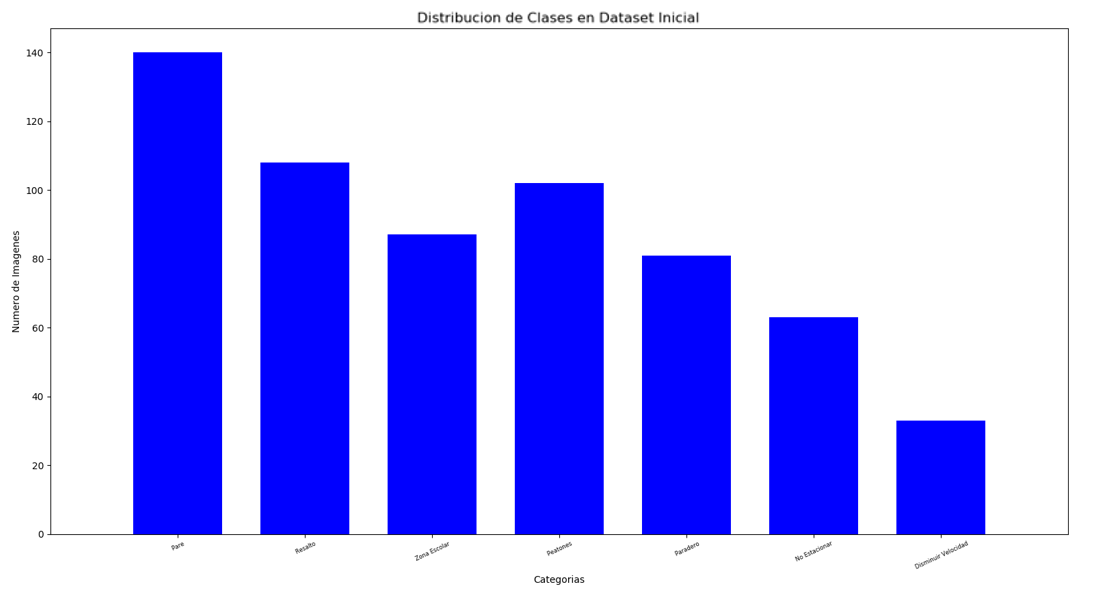
\includegraphics[width=1\textwidth]{images/desarrollo/histograms/inicioTrain614}
				\end{center}
				\begin{center}
				\caption{\small{Distribución de ejemplos por señal para el entrenamiento(Total 614)}}
				{\small{\fontsize{10}{16.8}\selectfont {Fuente: Elaboración propia}}}
				\end{center}
				\vspace{-1.5em}
			\end{figure}

			

	\subsection{Datos para el evaluación}
		Al igual que en el anterior punto, se obtienen un conjunto de menor cantidad de imágenes de señales de tránsito Alemán y Peruano, las cuales servirán para evaluar los modelos creados.

		\subsubsection{Señales de Tránsito de Alemania}
		Para la etapa de evaluación se cuenta con un conjunto de 12630 imágenes, de igual manera no necesariamente balanceadas y que no son utilizadas durante el proceso de entrenamiento para obtener resultados confiables a la hora de evaluar el resultado del entrenamiento. 

		\begin{figure}[H]
			%\begin{center}
			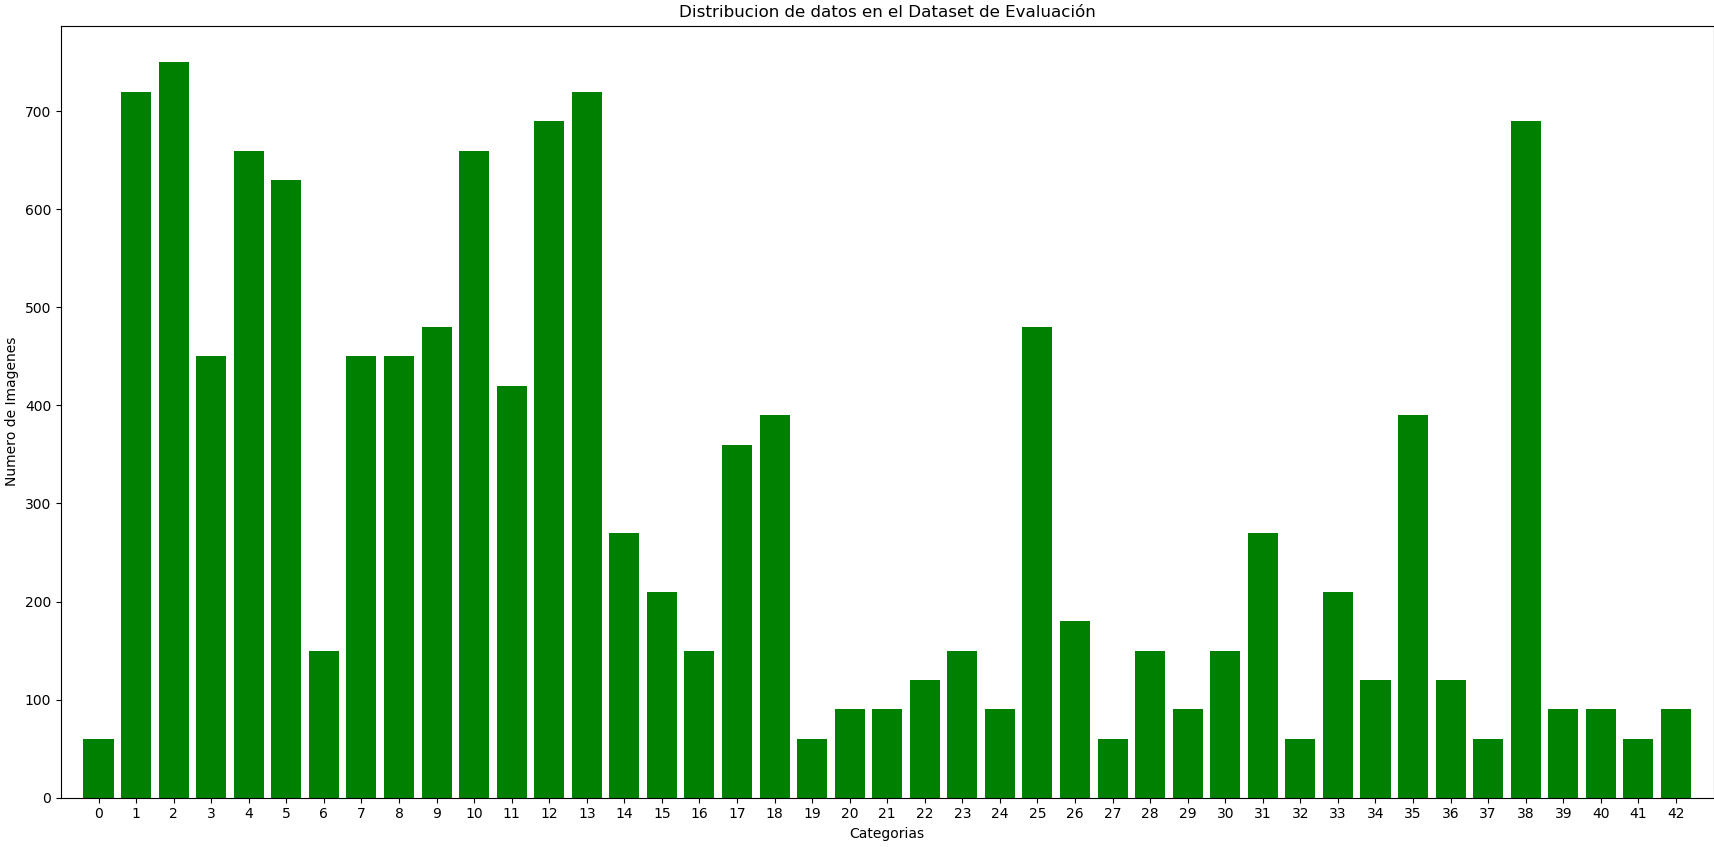
\includegraphics[width=1\textwidth]{images/desarrollo/histograms/initialTest12630}
			%\end{center}
			\begin{center}
			\caption{\small{Distribución de ejemplos por señal para la evaluación - Alemania}}
			{\small{\fontsize{10}{16.8}\selectfont {Fuente: Elaboración propia}}}
			\end{center}
			\vspace{-1.5em}
		\end{figure}

		\subsubsection{Señales de Tránsito de Perú}
		Para la etapa de evaluación se cuenta con un conjunto de 4698 imágenes, de igual manera no necesariamente balanceadas y que no son utilizadas durante el proceso de entrenamiento para obtener resultados confiables a la hora de evaluar el resultado del entrenamiento. 

		\begin{figure}[H]
			%\begin{center}
			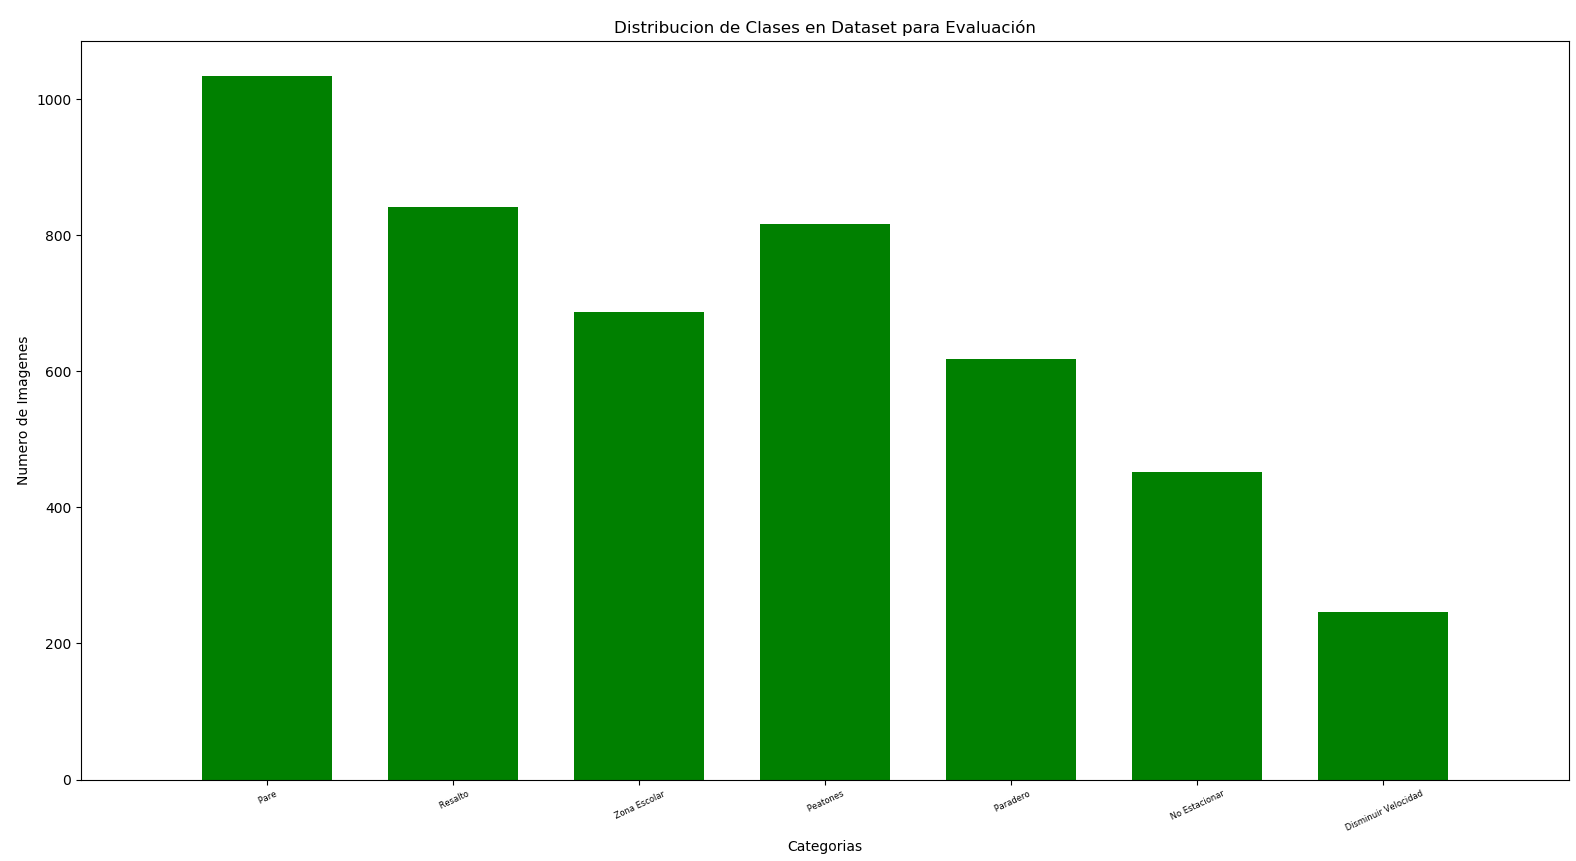
\includegraphics[width=1\textwidth]{images/desarrollo/histograms/PeruinitialTest4698}
			%\end{center}
			\begin{center}
			\caption{\small{Distribución de ejemplos por señal para la evaluación - Perú}}
			{\small{\fontsize{10}{16.8}\selectfont {Fuente: Elaboración propia}}}
			\end{center}
			\vspace{-1.5em}
		\end{figure}

	\subsection{Proceso de Aumento de Datos(Data Augmentation)}

		Las redes convolucionales durante el aprendizaje profundo requieren una gran cantidad de datos para conseguir realizar un mejor entrenamiento(aprendizaje) y obtener un modelo que generalice eficazmente. Muchas veces esta recopilación de datos suele ser costosa y laboriosa es por eso que el proceso de Data Augmentation ayuda a superar este problema a través del uso de métodos o técnicas de procesamiento de imágenes. Recientemente se ha utilizado ampliamente el aumento de datos genéricos para mejorar el rendimiento de las Redes Neuronales Convolucionales,\citep{DL_augmentData}. 

		\begin{figure}[H]
		\begin{center}
		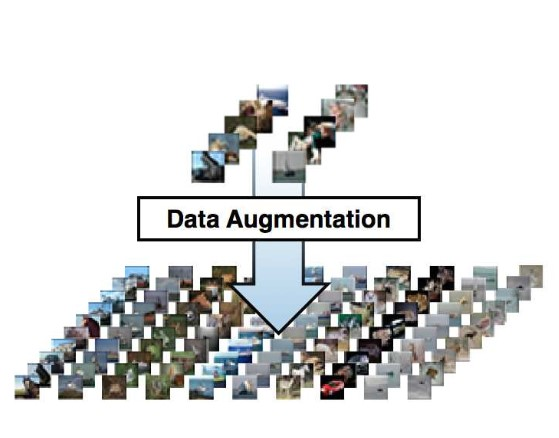
\includegraphics[width=0.5\textwidth ]{images/desarrollo/Augment/exampleaug}
		\end{center}
		\begin{center}
		\caption{\small{El aumento de datos infla artificialmente los conjuntos de datos usando transformaciones que preservan las categorias de los objetos}}
		{\small{\cite{DL_augmentData}}}
		\end{center}
		\vspace{-1.5em}
		\end{figure}


		Son utilizadas las siguientes técnicas:
		\begin{enumerate}
		\item[1)] Flipping (Horizontal/Vertical)
		\item[2)] Proyección
		\item[3)] Rotación
		\item[4)] Zoom (Out/In)
		\item[5)] Equialización de Histrogama
		\vskip 3cm
		\end{enumerate} 
		
		\subsubsection{Flipping}
		
			Primero, vamos a aplicar un par de trucos para extender nuestros datos volteando. Algunas señales de tráfico son invariantes para voltear horizontal y / o verticalmente, lo que básicamente significa que podemos voltear una imagen y todavía debe clasificarse como perteneciente a la misma clase.

			Esta técnica solo fue utilizada para el dataset de señales de Tránsito de Alemania.
			%\newpage
			\begin{multicols}{2}
				\underline{Flipping horizontal:}
				\vspace{-0.5cm}
				\begin{figure}[H]
					\begin{center}
					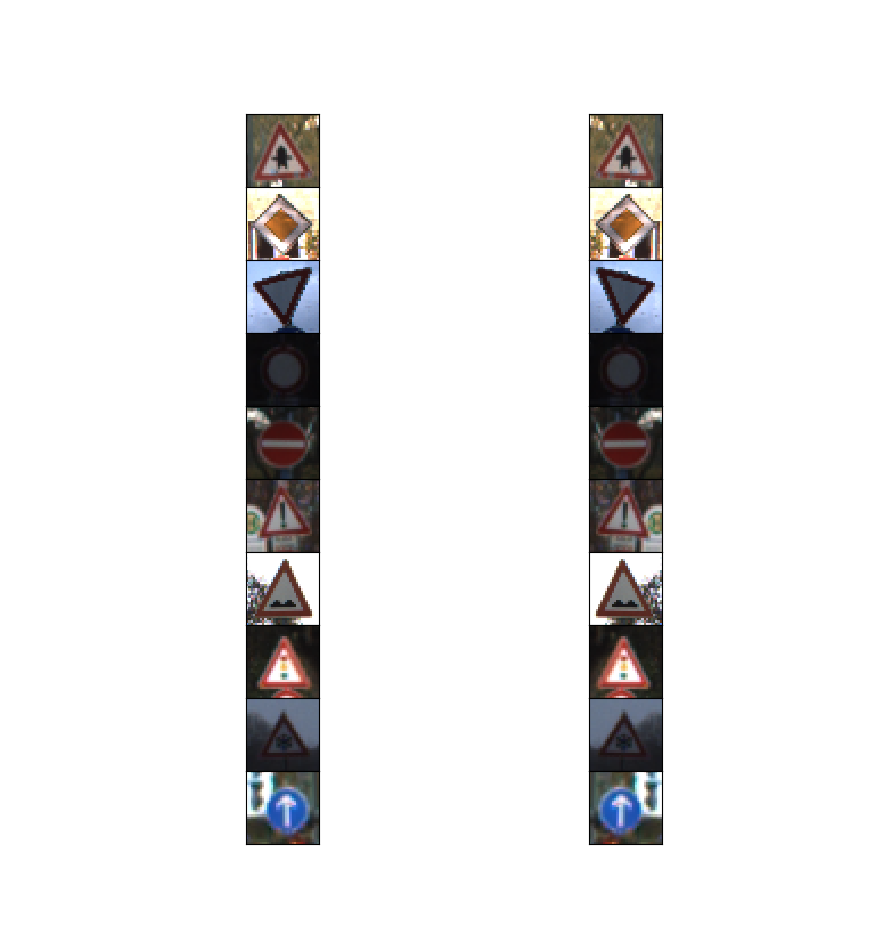
\includegraphics[height=10cm ]{images/desarrollo/Augment/flippedHorizontally}
					\end{center}
					\begin{center}
					\caption{\small{Imágenes volteadas horizontalmente}}
					{\small{\fontsize{10}{16.8}\selectfont {Fuente: Elaboración propia}}}
					\end{center}
					\vspace{-1.5em}
				\end{figure}

			%second column
			
				\underline{Flipping Vertical:}
				\begin{figure}[H]
					\begin{center}
					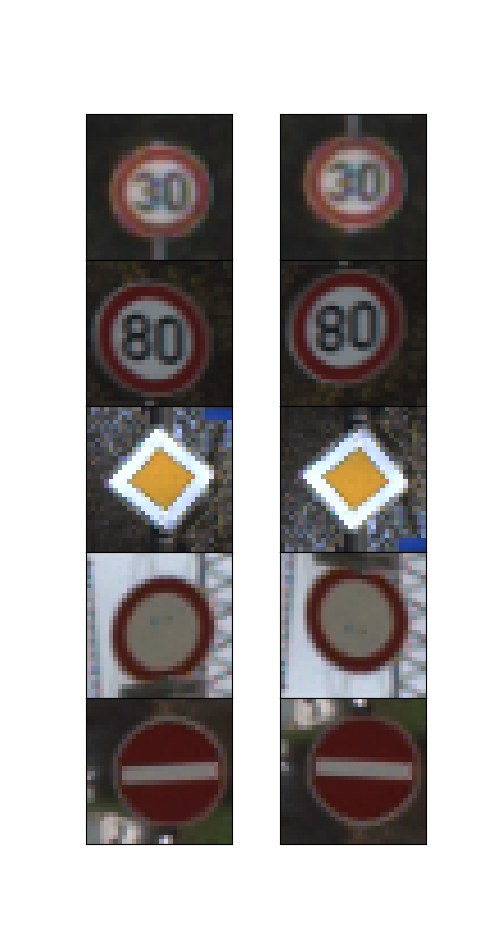
\includegraphics[height=10cm]{images/desarrollo/Augment/flippableVertically}
					\end{center}
					\begin{center}
					\caption{\small{Imágenes volteadas verticalmente}}
					
				{\small{\fontsize{10}{16.8}\selectfont {Fuente: Elaboración propia}}}
					\end{center}
					\vspace{-1.5em}
				\end{figure}

			\end{multicols}

			%\newpage
			\underline{Flipping Horizontal y Vertical:}
			\begin{figure}[H]
				\begin{center}
				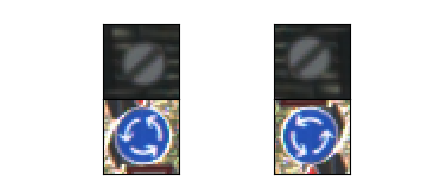
\includegraphics[width=0.5\textwidth, height=0.25\textheight]{images/desarrollo/Augment/flippable_both}
				%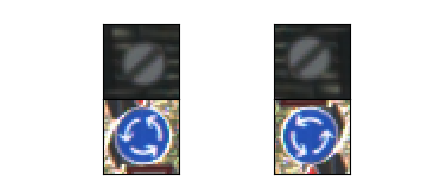
\includegraphics[height=4cm]{images/desarrollo/Augment/flippable_both}
				\end{center}
				\vspace{-1.em}
				\begin{center}
				\caption{\small{Imágenes volteadas primero horizontal y luego verticalmente}}
				{\small{\fontsize{10}{16.8}\selectfont {Fuente: Elaboración propia}}}
				\end{center}
				\vspace{-1.5em}
			\end{figure}

			Incluso, hay signos que luego de voltearse, deben clasificarse como un signo de alguna otra clase. Esto sigue siendo útil, ya que podemos utilizar los datos de estas clases para ampliar sus contrapartes.
			\begin{figure}[H]
				\begin{center}
				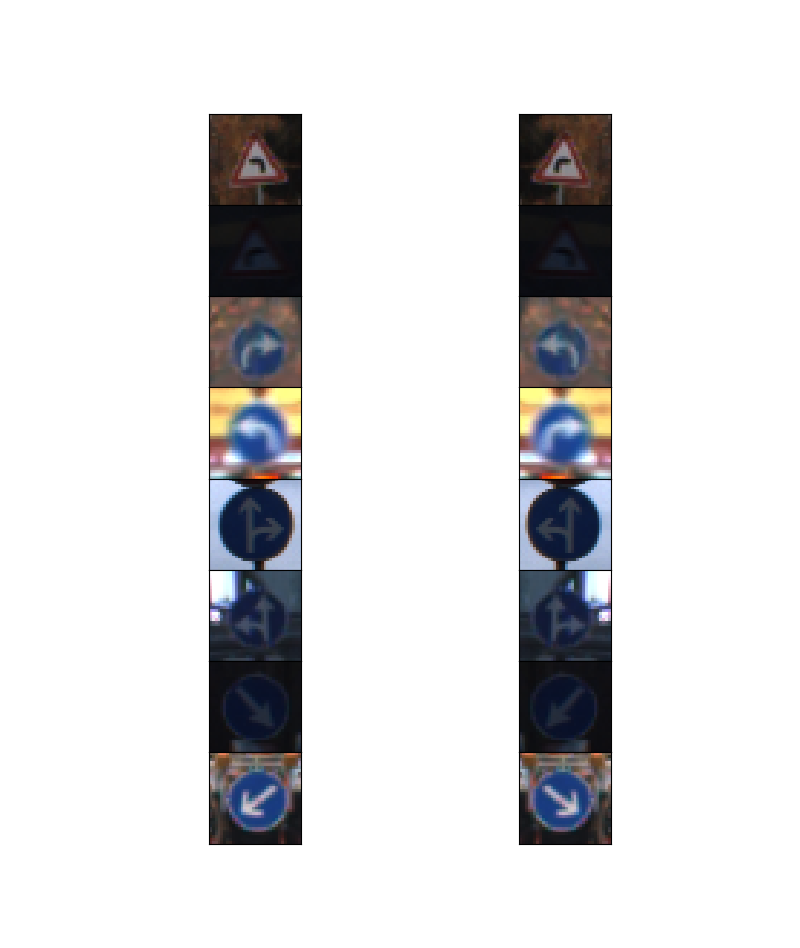
\includegraphics[width=5cm ,height=8.5cm ]{images/desarrollo/Augment/cross_flippable}
				\end{center}
				\begin{center}
				\caption{\small{Imágenes que volteadas horizontal o verticalmente, cambian su categoría}}		
				{\small{\fontsize{10}{16.8}\selectfont {Fuente: Elaboración propia}}}
				\end{center}
				\vspace{-1.5em}
			\end{figure}


			Finalmente obtenemos una nueva distribución de datos luego de haber aplicado flipping a ciertas imagenes. Esta distribución consta de 63538 imágenes.
			\begin{figure}[H]
				\begin{center}
				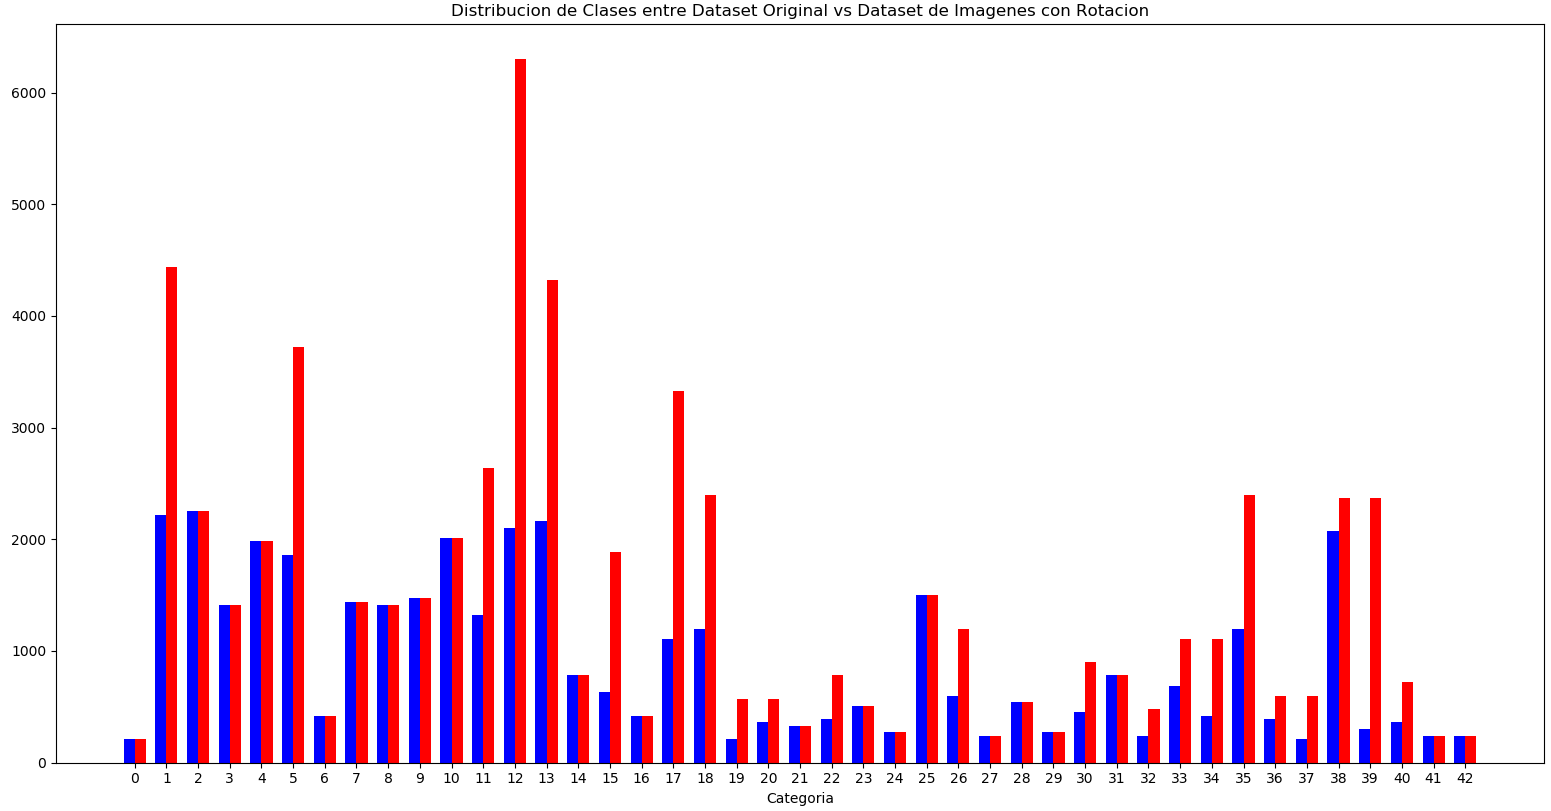
\includegraphics[width=1\textwidth]{images/desarrollo/histograms/train_flipped63538}
				\end{center}
				\begin{center}
				\vspace{1em}
				\caption{\small{Distribución de categoría, luego de aplicar el Flip(en sus distintos tipos)- Señales de Alemania}}
				{\small{\fontsize{10}{16.8}\selectfont {Fuente: Elaboración propia}}}
				\end{center}
				\vspace{-1.5em}
			\end{figure}

		A excepción de esta técnica, las siguientes fueron utilizadas para ambos datasets de imágenes (Alemania y Perú).
		
		\subsubsection{Projection(Proyección)}
			Implica mover la imagen a lo largo de la dirección X o Y (o ambas). Este método de aumento es muy útil ya que la mayoría de los objetos se pueden ubicar en casi cualquier lugar de la imagen, obligando a la red neuronal convolucional a buscar en todas partes. Los márgenes de proyección se asignan al azar en un rango que depende del tamaño de la imagen. La transformación de proyección también se ocupar de escalar al azar a medida que colocamos al azar las esquinas de la imagen en un rango [-delta, +delta].

			\begin{figure}[H]
				\begin{center}
				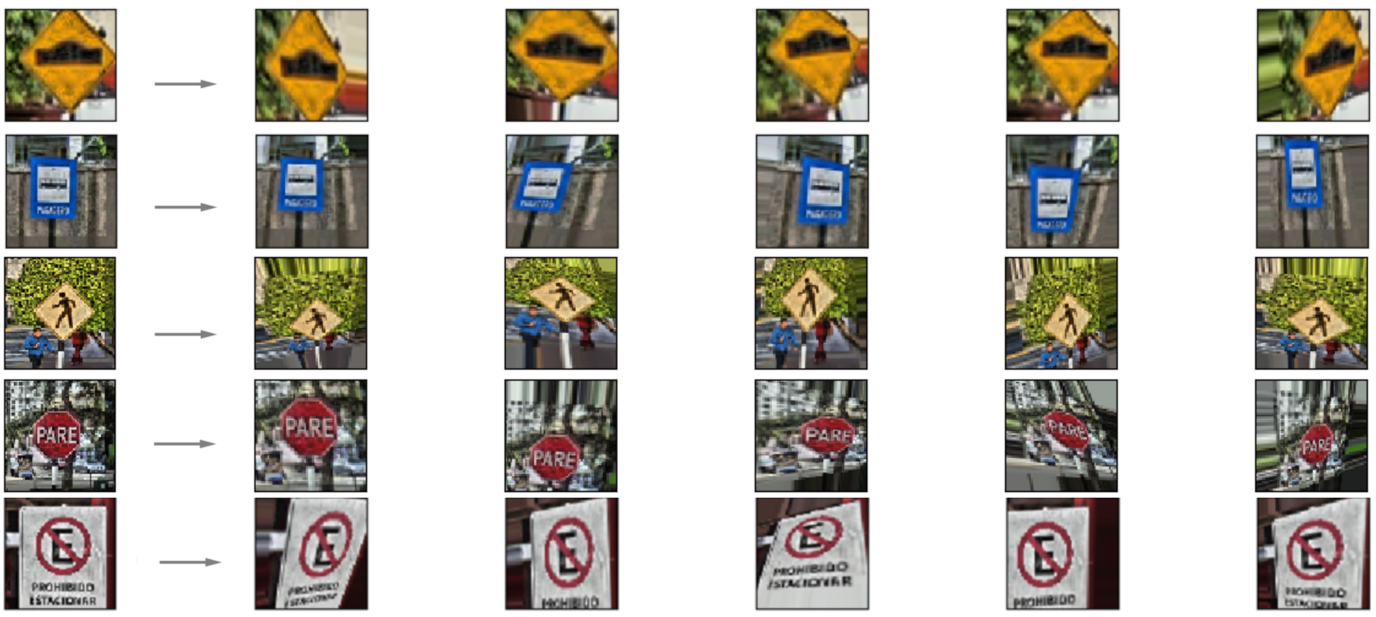
\includegraphics[width=1\textwidth,height=7.5cm]{images/desarrollo/Augment/projection_transform3}
				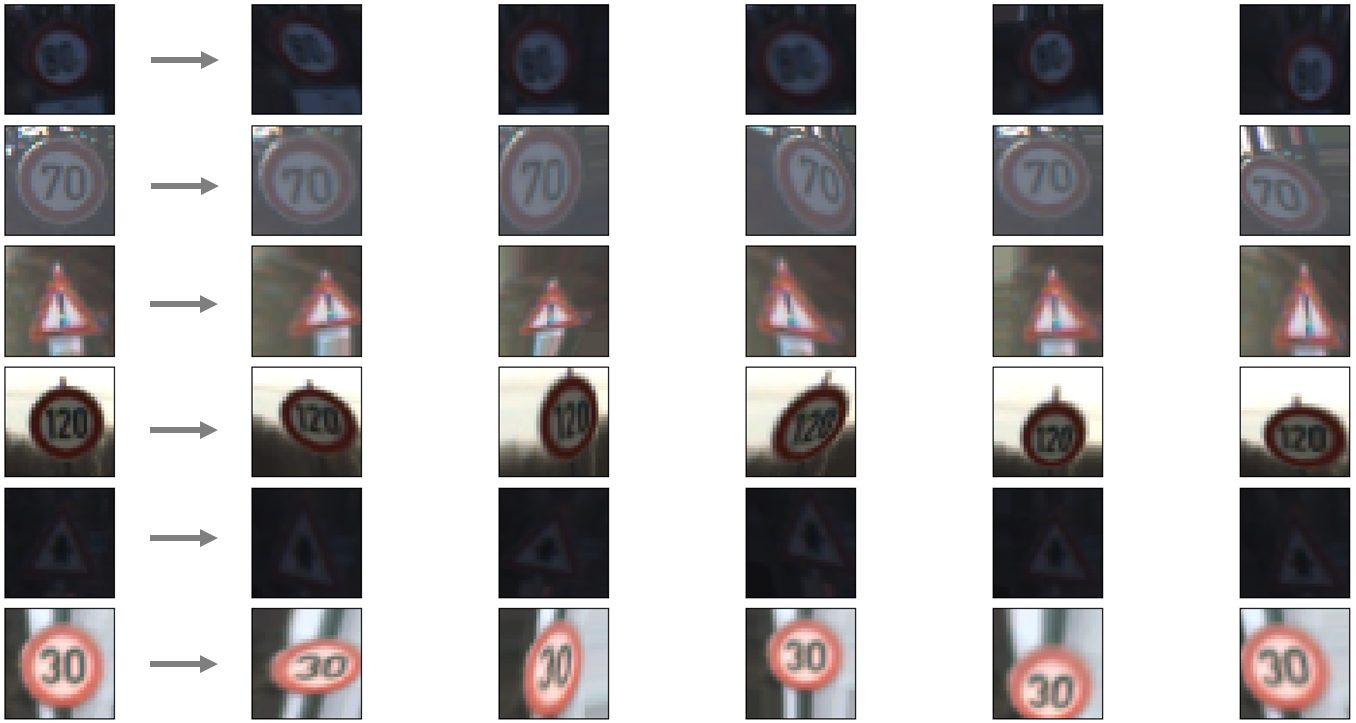
\includegraphics[width=1\textwidth,height=7.5cm]{images/desarrollo/Augment/projection_transform}
				\end{center}
				\begin{center}
				\vspace{1em}
				\caption{\small{Ejemplo de cinco proyecciones por imagen - Dataset Perú y Alemania}}	
				{\small{\fontsize{10}{16.8}\selectfont {Fuente: Elaboración propia}}}
				\end{center}
				\vspace{-1.5em}
			\end{figure}
		\newpage
		\subsubsection{Rotation(Rotación)}
			%\vspace{-1.5em}
			Aplica la rotación aleatoria en un rango de grados definido(hasta 30º) a un subconjunto aleatorio de imágenes.
	        El rango en sí está sujeto a escala dependiendo de la intensidad de aumento.

	        \begin{figure}[H]
				\begin{center}
				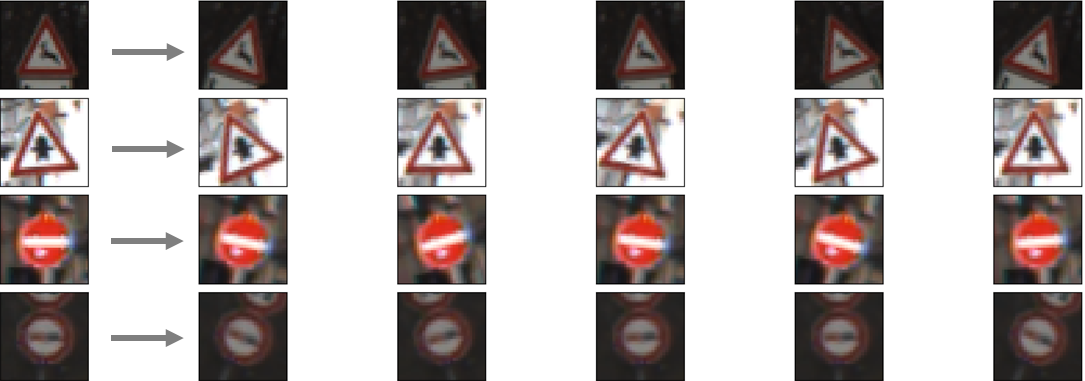
\includegraphics[width=1\textwidth,height=6cm]{images/desarrollo/Augment/fixedrotation3}
				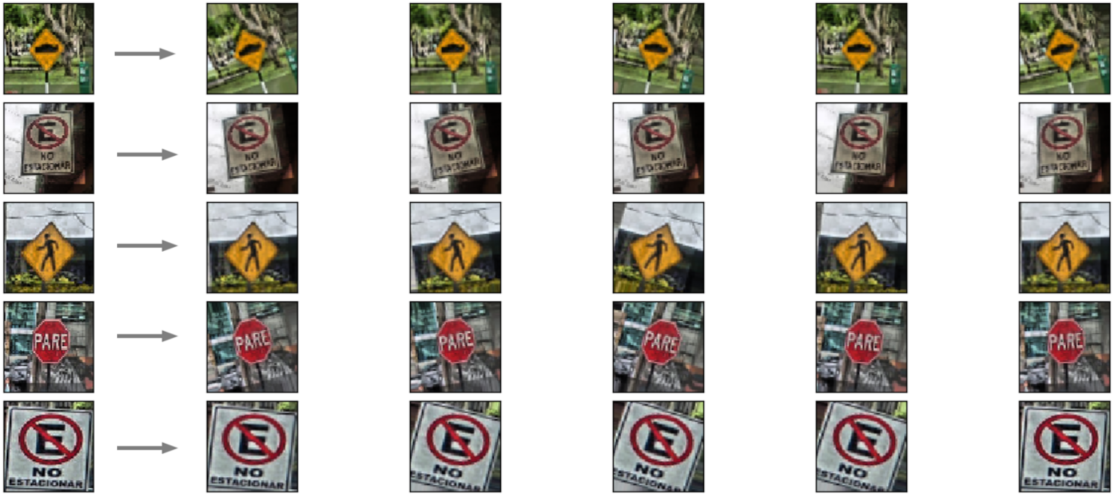
\includegraphics[width=1\textwidth,height=9cm]{images/desarrollo/Augment/fixedrotation2}
				\end{center}
				\begin{center}
				\caption{\small{Ejemplo de cinco rotaciones por imagen - Dataset Alemania y Perú}}
				{\small{\fontsize{10}{16.8}\selectfont {Fuente: Elaboración propia}}}
				\end{center}
				\vspace{-1.5em}
			\end{figure}
			%\vspace{-2.5em}
	    
		\newpage
	    \subsubsection{Zoom}
	    	%\vspace{-1.5em}
	    	Acerca(zoom in) o aleja(zoom out) la imagen  tratando de preservar el fondo.

	    	%\begin{figure}[H]
			%	\begin{center}
			%	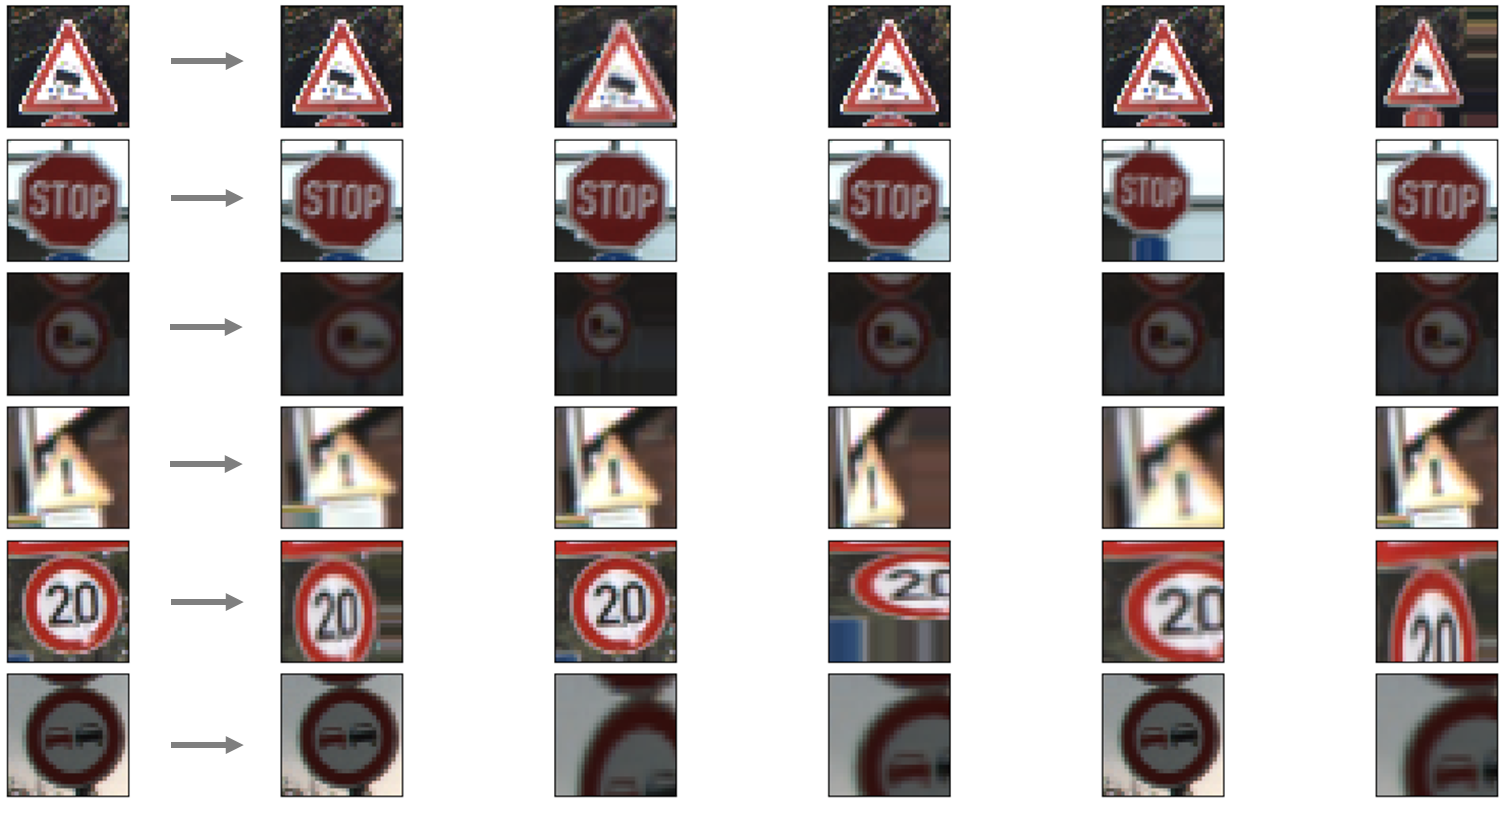
\includegraphics[width=1\textwidth,height=10cm]{images/desarrollo/Augment/zoom_normal}
			%	\end{center}
			%\end{figure}

			\begin{figure}[H]
				\begin{center}
				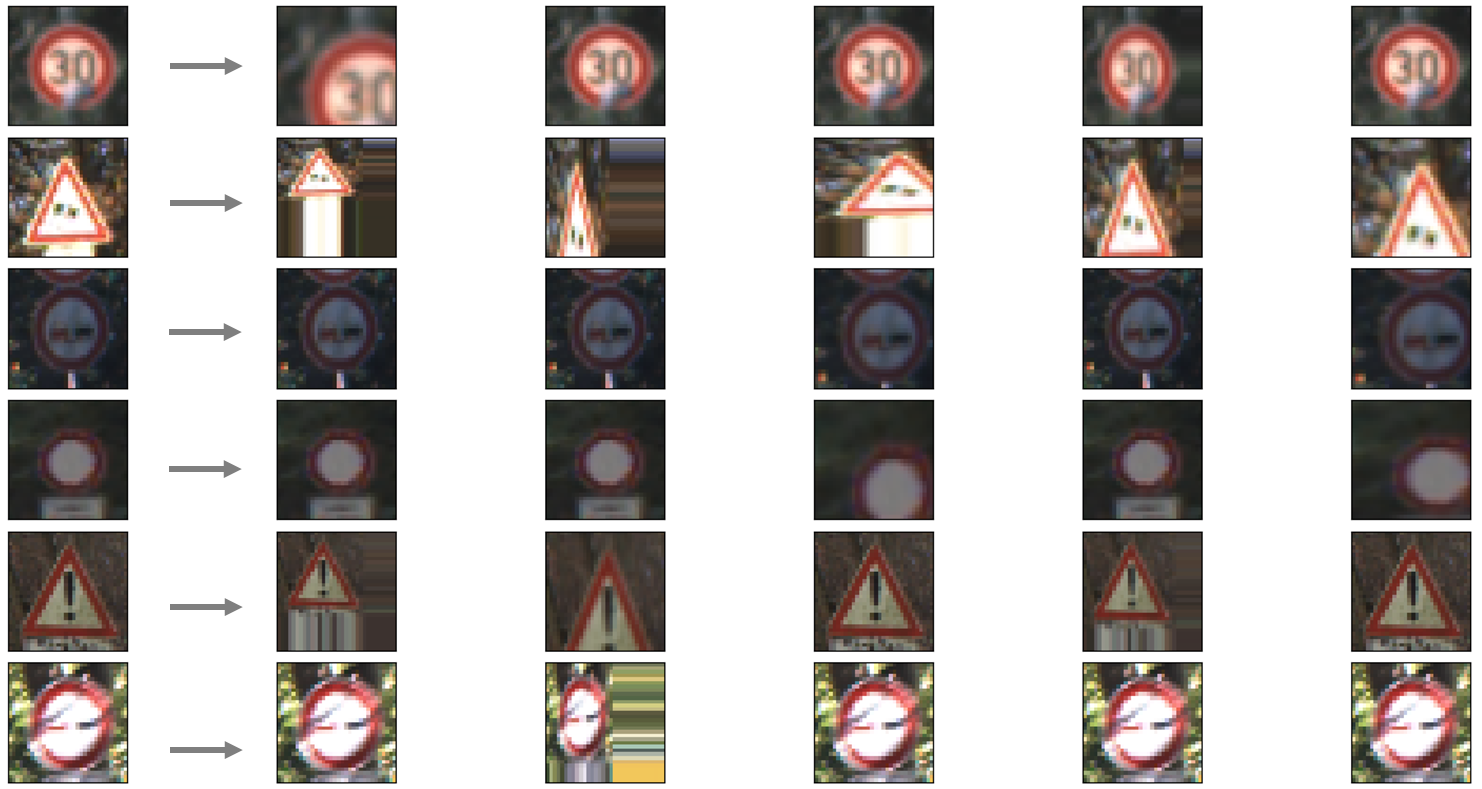
\includegraphics[width=1\textwidth,height=7.5cm]{images/desarrollo/Augment/zoom_inv}
				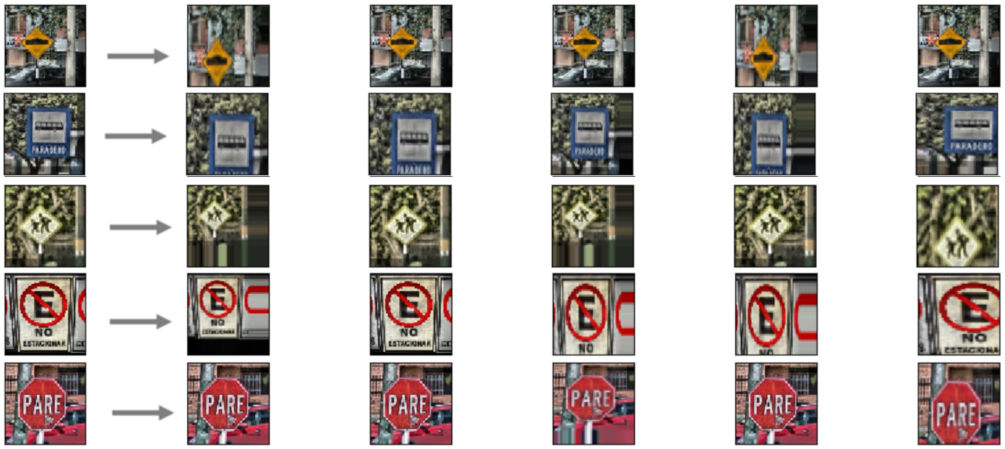
\includegraphics[width=1\textwidth,height=7.5cm]{images/desarrollo/Augment/zoom_inv2}
				\end{center}
				\begin{center}
				\vspace{0.5em}
				\caption{\small{Ejemplo de cinco aplicaciones de zoom(in/out) por cada imagen - Dataset Alemania y Perú}}
				{\small{\fontsize{10}{16.8}\selectfont {Fuente: Elaboración propia}}}
				\end{center}
				\vspace{-1.5em}
			\end{figure}

		\vspace{1.5em}
		\subsubsection{Equalizacion del histograma}
			Aumenta el contraste global de muchas imágenes, especialmente cuando los datos utilizables de la imagen están representados por valores de contraste cercanos. Esto permite que áreas de menor contraste local puedan obtener un mayor contraste. La ecualización del histograma logra esto al distribuir eficazmente los valores de intensidad más frecuentes.

			\begin{figure}[H]
				\begin{center}
				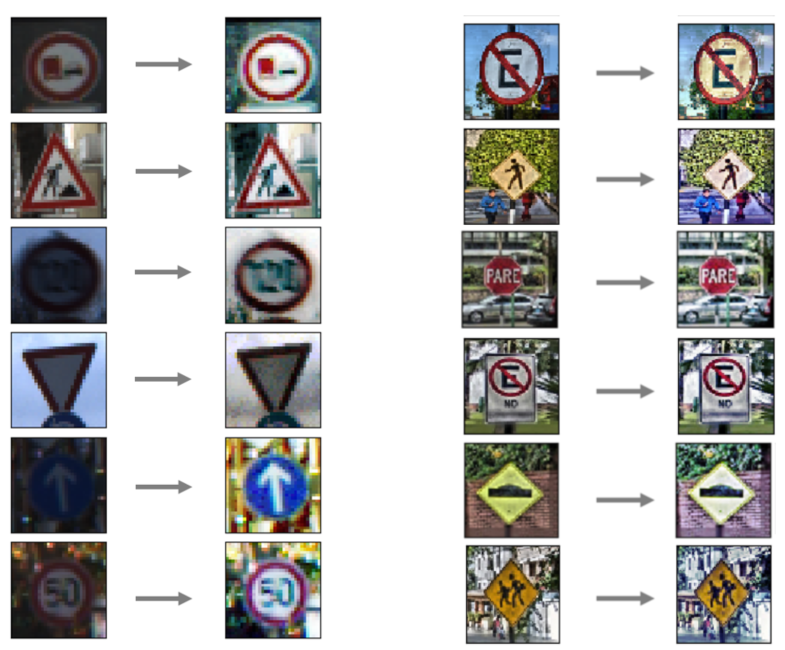
\includegraphics[height=11.5cm]{images/desarrollo/Augment/equalize_hist2_wo_Norm_woRepetition2}
				\end{center}
				\begin{center}
				\caption{\small{Distribución eficaz de los valores de intensidad más frecuentes}}
				{\small{\fontsize{10}{16.8}\selectfont {Fuente: Elaboración propia}}}
				\end{center}
				\vspace{-1.5em}
			\end{figure}
		
		
		%	\begin{figure}[H]
				%\begin{center}
		%		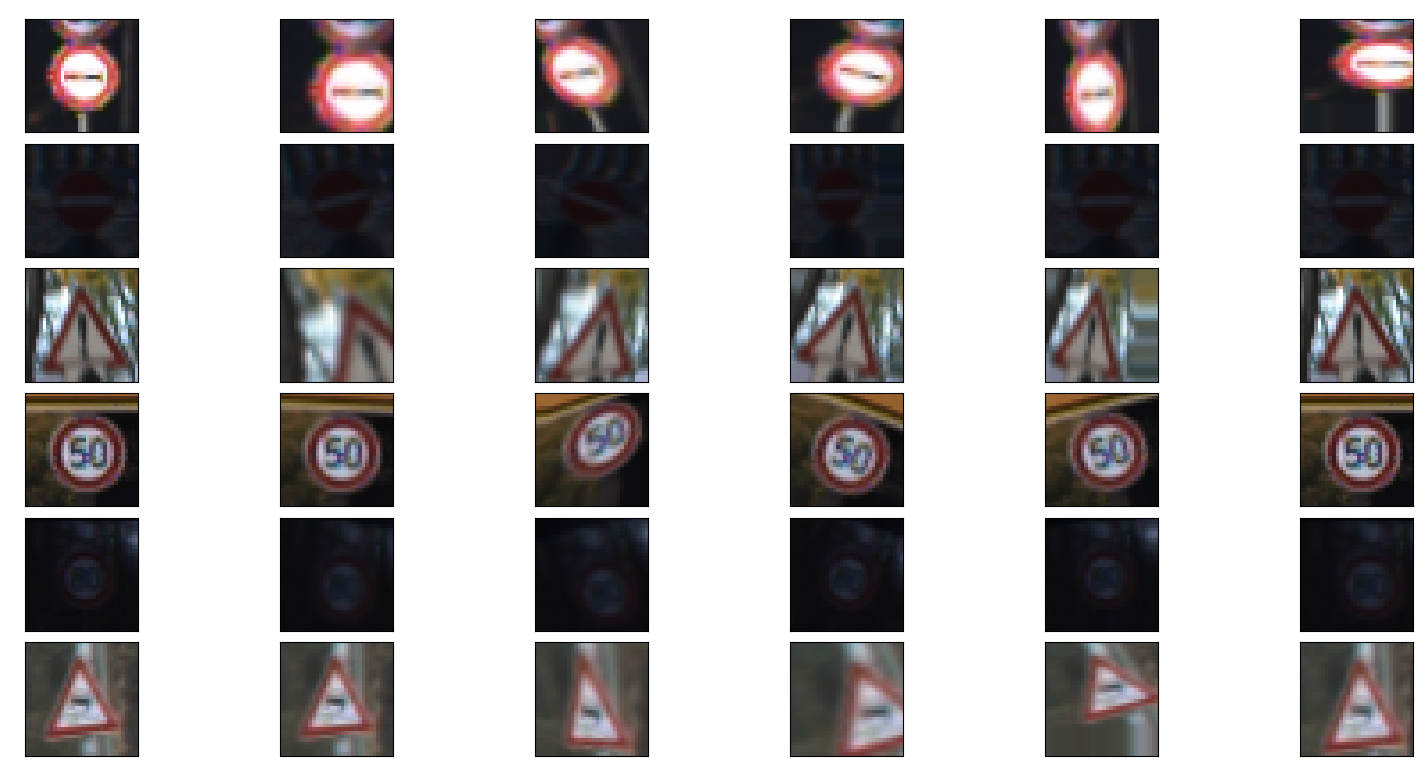
\includegraphics[width=0.9\textwidth,height=11cm]{images/desarrollo/Augment/AllTogether_ramdoly_mixed2}
				%\end{center}
		%		\begin{center}
		%		\caption{\small{Ilustración de un modelo de aprendizaje profundo}}
		%		
		%	{\small{\fontsize{10}{16.8}\selectfont {Fuente: Elaboración propia}}}
		%		\end{center}
		%		\vspace{-1.5em}
		%	\end{figure}

	\newpage
	\subsection{Dataset final para el Entrenamiento}
		Finalmente, luego de haber aplicado de manera secuencial y/o aleatoriamente estas técnicas a cada una de las imágenes, obtenemos nuevas distribuciones de datos. 
		\subsubsection{Señales de Tránsito de Alemania - Dataset Balanceado }
			En una se tiene un conjunto balanceado de datos con {\bf 270900 imágenes}.
			\begin{figure}[H]
				%\begin{center}
				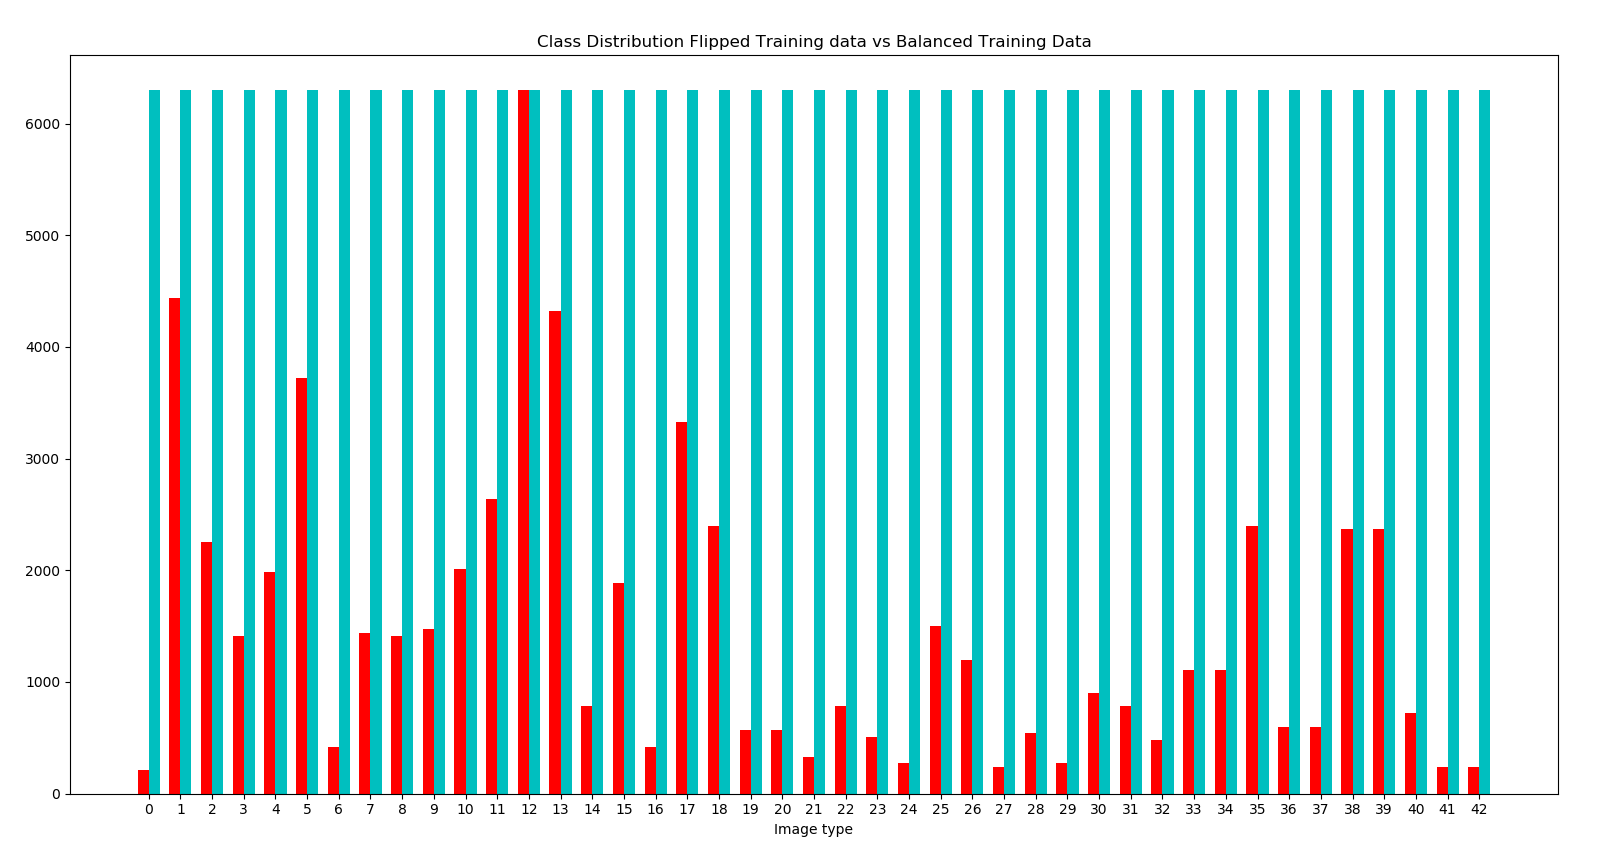
\includegraphics[width=1\textwidth, height=8.5cm]{images/desarrollo/histograms/train_extended_balanced270900}
				%\end{center}
				\begin{center}
				\caption{\small{Dataset balanceado(cada categoría posee igual cantidad de imágenes)}}
				{\small{\fontsize{10}{16.8}\selectfont {Fuente: Elaboración propia}}}
				\end{center}

			\end{figure}

			Teniendo en cuenta lo descrito en la \textbf{Seccion 2.3.4 (Validación Cruzada)}, para la etapa del entrenamiento, el conjunto de datos Balanceados compuesto por 270900 imágenes fue dividido en un subconjunto de entrenamiento y otro para validación, con la siguiente distribución:
			\vspace{1.5em}
			\begin{table}[H]
				\caption{\small{Distribución Entrenamiento y Validación Dataset Balanceado - Señales de Tránsito de Alemania}}
				\begin{center}
				\begin{tabular}{|>{\scriptsize}c|>{\scriptsize}c|}
				\hline
				{\ul \textbf{CONJUNTO DE DATOS}}           & {\ul \textbf{CANTIDAD IMÁGENES}}                \\ \hline
				\textbf{Entrenamiento}                    & \text{203175 (75\%)}                       \\ \hline
				\textbf{Validación}                       & \text{67725 (25\%)}                    \\ \hline
				\end{tabular}
				\end{center}
			\end{table}

	%---------------------------------------------------------------------------------------------------------------------------------------------------------
	
		\subsubsection{Señales de Tránsito de Perú - Dataset No Balanceado}
			Con el objetivo de obtener una gran cantidad de datos, para el Dataset de señales de Tránsito del Perú, por cada imágen fueron creadas 50 nuevas imágenes, obteniéndose {\bf 31314 imágenes}.
			\begin{figure}[H]
				%\begin{center}
				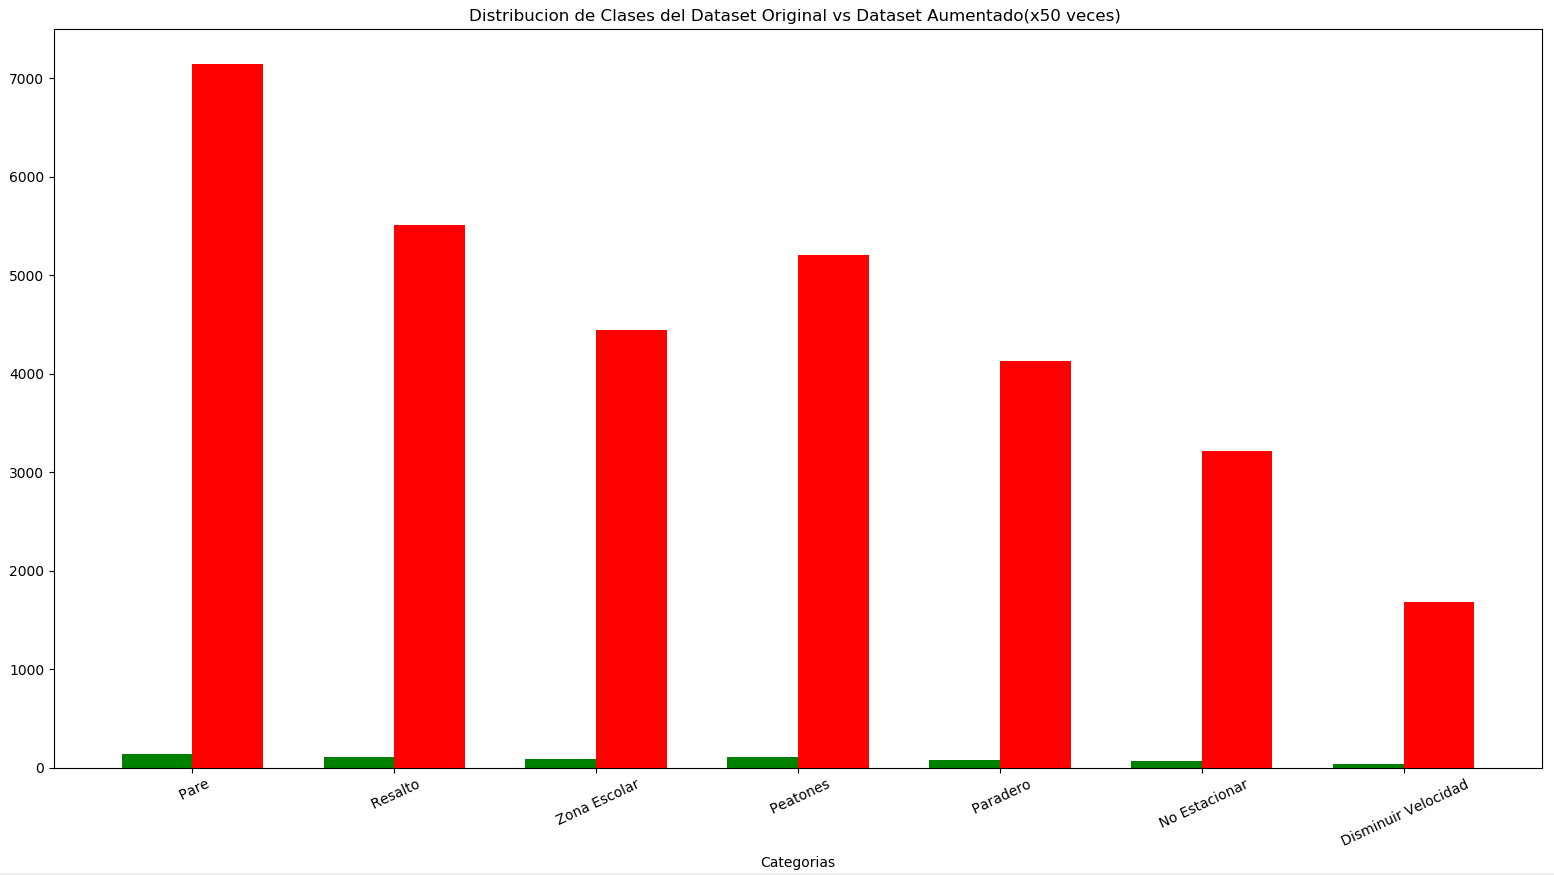
\includegraphics[width=1\textwidth, height=8.5cm]{images/desarrollo/histograms/train_extended_per_51_31314}
				%\end{center}
				\begin{center}
				\caption{\small{Dataset no balanceado - Señales de Tránsito de Perú}}
				
				{\small{\fontsize{10}{16.8}\selectfont {Fuente: Elaboración propia}}}
				\end{center}
			\end{figure}

			Para este caso, el dataset aumentado se configuró con una distribución de datos para entrenamiento, validación y evaluación: 
			\vspace{1.5em}
			\begin{table}[H]
				\caption{\small{Distribución Entrenamiento y Validación Dataset no Balanceado - Señales de Tránsito de Perú}}
				\begin{center}
				\begin{tabular}{|>{\scriptsize}c|>{\scriptsize}c|}
				\hline
				{\ul \textbf{CONJUNTO DE DATOS}}           & {\ul \textbf{CANTIDAD IMÁGENES}}     \\ \hline
				\textbf{Entrenamiento}                    & \text{23485 (75\%)}                   \\ \hline
				\textbf{Validación}                       & \text{3131 (10\%)}                    \\ \hline
				\textbf{Evaluación}                       & \text{4698 (15\%)}                    \\ \hline
				\end{tabular}
				\end{center}
			\end{table}

	%---------------------------------------------------------------------------------------------------------------------------------------------------------
	%\newpage
	\subsection{Pre-procesamiento de Imágenes(Normalization)}
		Existe una técnica de procesamiento de imágenes por computadora que se utiliza para mejorar el contraste en las imágenes denominada Ecualización Adaptativa del Histograma(AHE por sus siglas en inglés). Difiere de la ecualización de histograma ordinaria en el sentido de que el método adaptativo computa varios histogramas, cada uno correspondiente a una sección distinta de la imagen, y los utiliza para redistribuir los valores de luminosidad de la imagen. Por lo tanto, es adecuado para mejorar el contraste local y mejorar las definiciones de los bordes en cada región de una imagen. Sin embargo, AHE tiene una tendencia a amplificar el ruido en regiones relativamente homogéneas de una imagen. Una variante de la ecualización de histograma adaptativo llamada ecualización de histograma adaptativo limitado por contraste (CLAHE por sus siglas en inglés) evita que se genere esto al limitar la amplificación.

		En esta investigación, aplicaremos la técnica CLAHE, un algoritmo para la mejora del contraste local, que utiliza histogramas calculados sobre diferentes regiones en una imagen. Utilizado frecuentemente para mejorar el nivel de visibilidad de una imagen o video con niebla ya que permite mejorar los detalles locales incluso en regiones que son más oscuras o más claras que la mayoría de regiones de la imagen. Este algoritmo mejorará aún más la extracción de características de cada imágen.\citep{CLAHE}

			\begin{figure}[H]
			%\begin{center}
			
\includegraphics[width=1\textwidth]{images/desarrollo/Normalization_Processing/norm_test1}
			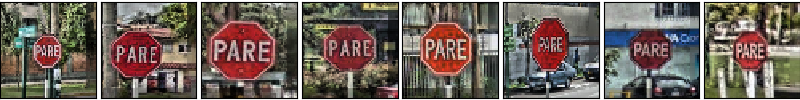
\includegraphics[width=1\textwidth]{images/desarrollo/Normalization_Processing/norm_test3}
			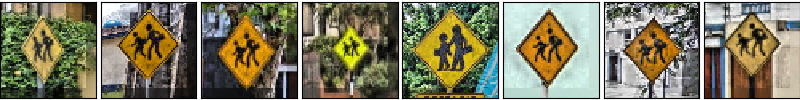
\includegraphics[width=1\textwidth]{images/desarrollo/Normalization_Processing/norm_test4}
			%\end{center}
			\begin{center}
			\caption{\small{Imágenes a las cuales se le aplicaron la técnica CLAHE }}
			
			{\small{\fontsize{10}{16.8}\selectfont {Fuente: Elaboración propia}}}
			\end{center}
			\vspace{-1.5em}
			\end{figure}
		
		Por otra parte, para convertir un color de un espacio de color basado en un modelo de color RGB típico de gamma comprimido (no lineal) a una representación en escala de grises de su luminancia, primero se debe eliminar la función de compresión gamma mediante la expansión gamma (linealización) para transformar la imagen en un RGB lineal espacio de color, de modo que la suma ponderada apropiada se puede aplicar a los componentes de color lineales ($R_{linear} , G_{linear} , B_{linear}$) para calcular la luminancia lineal $Y_{linear}$.

		Para imágenes en espacios de color como Y'UV y sus derivados, que se usan en sistemas de TV y video a color estándar como PAL, SECAM y NTSC, un componente de luma no lineal ($Y'$) se calcula directamente a partir de intensidades primarias comprimidas con gamma como una suma ponderada, que aunque no es una representación perfecta de la luminancia colorimétrica, puede calcularse más rápidamente sin la expansión gamma y sin la compresión utilizadas en los cálculos fotométricos o colorimétricos,\citep{POYNTON2003257}. En los modelos utilizados por PAL y NTSC para conseguir tener las imágenes en escala de grises, el componente de luma no lineal ($Y'$) se calcula como: \begingroup\makeatletter\def\f@size{14.8}\check@mathfonts	$Y' = 0.299R' + 0.587G' +0.114B'$ \endgroup \citep{CookJ}

		Pierre Sermanet y Yann LeCun mencionaron en su artículo \citep{LeCun}, que el uso de canales de color no pareció mejorar mucho las cosas. Además, debido a diversas condiciones o problemas de iluminación, no es adecuado procesar directamente las imágenes que se capturan a través de la cámara o sensores de imágenes, es por ello que en esta investigación {\bf se usará un solo canal} en el modelo, es decir las imágenes estarán en escala de grises en lugar de tener 3 canales de colores.
		
			\begin{figure}[H]
			\begin{center}
			
\includegraphics[width=0.7\textwidth]{images/desarrollo/Normalization_Processing/proc_test1}
			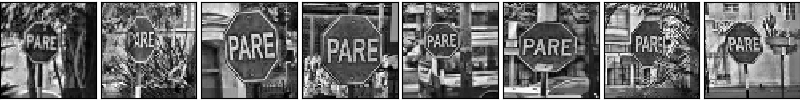
\includegraphics[width=0.7\textwidth]{images/desarrollo/Normalization_Processing/proc_test3}
			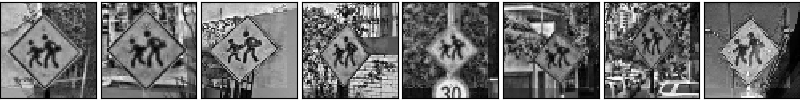
\includegraphics[width=0.7\textwidth]{images/desarrollo/Normalization_Processing/proc_test4}
			\end{center}
			\begin{center}
			\caption{\small{Imágenes procesadas en escala de grises}}
			
			{\small{\fontsize{10}{16.8}\selectfont {Fuente: Elaboración propia}}}
			\end{center}
			\vspace{-1.5em}
			\end{figure}
			\newpage
	

\section{Arquitectura del Modelo}


	Los hiperparámetros engloban funciones, variables y constantes utilizadas durante la construcción de las diferentes arquitecturas; estas varían, sin embargo siguiendo conceptos teóricos, antecedentes(investigaciones previas) y sobretodo despues de algunas pruebas realizadas, los siguientes hiperparámetros fueron seleccionados de manera específica:
		% Please add the following required packages to your document preamble:
		% \usepackage{multirow}
		%\usepackage[table,xcdraw]{xcolor}
		% If you use beamer only pass "xcolor=table" option, i.e. \documentclass[xcolor=table]{beamer}
		% \usepackage[normalem]{ulem}
		% \useunder{\uline}{\ul}{}
		\begin{table}[H]
			\begin{center}
			\caption{\small{Hiperparámetros del Modelo}}
			\begin{tabular}{|>{\scriptsize}c|>{\scriptsize}c|>{\scriptsize}c|>{\scriptsize}c|}
			\hline
			{\ul \textbf{HIPERPARÁMETROS}}  & {\ul \textbf{TIPO}}       & {\ul \textbf{HIPERPARÁMETROS}}        & {\ul \textbf{TIPO}}        \\ \hline
			{\textbf{Inicialización de Pesos}}                     		& {\textit{Xavier}}  				  &
			\textbf{Tasa de Aprendizaje}                                & \textit{0.0005}                    \\ \hline
			\textbf{Alg. de Optimización}                               & \textit{Optimizador Adam}          &
			\textbf{Método de Validación}                               & \textit{Entropía Cruzada}          \\ \hline
			\textbf{Fun. Activ. Capas Convolucionales}        			& \textit{RELU y DropOut}                      &
			\textbf{Fun. Activ. Capas Totalmente Conectadas} 			& \textit{Func. Softmax}           \\ \hline
			\textbf{Método de Regularización}                           &\textit{L2 Lasso(lambda = 0.0001)} &
			\textbf{Épocas}                                             &\textit{100}		 				\\ \hline
			\end{tabular}
			\end{center}
		\end{table}
		\vspace{-1.5em}

		Recordemos que en cada época se procesa el dataset completo de imágenes, por lo que cada época es igual : \begingroup\makeatletter\def\f@size{11}\check@mathfonts	$Epoca = \text{\textit{Tamaño del Minibatch}} \times \text{\textit{iteraciones}}$ \endgroup

		Sin embargo debido a que se tiene dos distintos datasets para el entrenamiento \textbf{(Seccion 3.1.4 - Dataset final para el Entrenamiento)}, el tamaño del Minibatch cambiará respecto al tamaño del dataset y por ende también será diferente la cantidad de iteraciones ejecutadas durante 100 épocas de entrenamiento. 

		A continuación se presentan 2 cuadros con las distribuciones del tamaño del Mini-batch y la cantidad de iteraciones necesarias durante las 100 épocas para ambos tipos de dataset(Alemania y Perú).                
		
		%\begin{center}\end{center}

		\begin{table}[H]
			\begin{center}
			\caption{\small{Minibatch e iteraciones en el Dataset de Señales de Tránsito de Alemania Balanceado}}
			\begin{tabular}{|>{\scriptsize}c|>{\scriptsize}c|>{\scriptsize}c|>{\scriptsize}c|}
			\hline
			\textbf{Imágenes totales }                 &\textit{203175}                       \\ \hline
			\textbf{Iteraciones por Época}                 &\textit{387}                             \\ \hline
			\textbf{Tamaño del Mini-batch}                 &\textit{525 imágenes analizadas por iteración}                       \\ \hline
			\textbf{Épocas entrenadas}                &\textit{100 épocas (38700 iter.)}                       \\ \hline
			\end{tabular}
			\end{center}
		\end{table}


		\begin{table}[H]
			\begin{center}
			\caption{\small{Minibatch e iteraciones en el Dataset de Señales de Tránsito de Peru No Balanceado}}
			\begin{tabular}{|>{\scriptsize}c|>{\scriptsize}c|>{\scriptsize}c|>{\scriptsize}c|}
			\hline
			\textbf{Imágenes totales }                 &\textit{23485}                       \\ \hline
			\textbf{Iteraciones por Época}                 &\textit{77}                             \\ \hline
			\textbf{Tamaño del Mini-batch}                 &\textit{305 imágenes analizadas por iteración}                       \\ \hline
			\textbf{Épocas entrenadas}                &\textit{100 épocas (7700 iter.)}                       \\ \hline
			\end{tabular}
			\end{center}
		\end{table}



	En esta investigación se implementó el modelo de redes neuronales convolucionales(CNN) donde las capas convolucionales iniciales de la red extraen características de la imagen(feature extractor), mientras que las capas totalmente conectadas predicen las probabilidades de salida(classifier).

	\begin{figure}[H]
		\begin{center}
		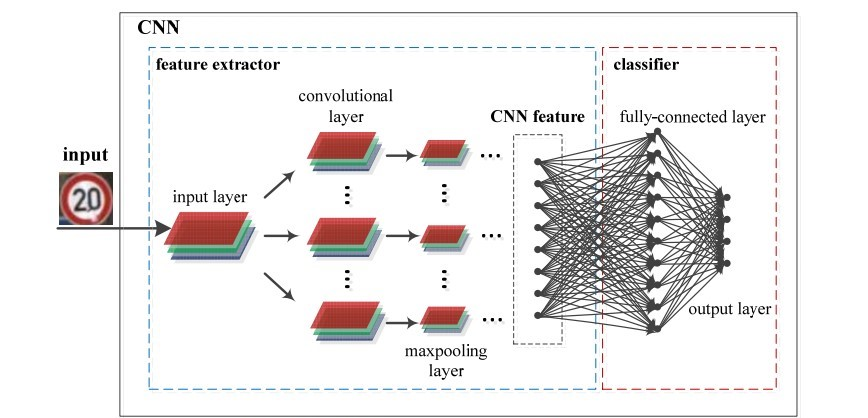
\includegraphics[width=0.8\textwidth]{images/desarrollo/networkArquitec/tempGeneralCNNmodel}
		\end{center}
		\begin{center}
		\caption{\small{Arquitectura de la CNN}}
		{\small{Fuente: \cite{ExtremeLearning}}}
		\end{center}
		\vspace{-1.5em}
	\end{figure}
	
	La arquitectura de la red está inspirada en el arquitectura Inception \citep{Inception} y en la arquitectura AlexNet \citep{Krizhevsky2012} para la clasificación de imágenes. En la arquitectura Inception, el modelo creado es denominado GoogLeNet, similar a AlexNet donde varios módulos iniciales son apilados uno sobre el otro para producir el resultado final. En el módulo de inicio, en ese tipo de red se usaron diversos tamaños de filtros convolucionales para capturar características de diferente abstracción. El alto nivel de abstracción se captura con filtros de mayor tamaño y el de un nivel inferior con filtros de menor tamaño, procesando información visual a diferentes escalas y al concatenarlas se obtiene un nivel eficiente de abstracción. 
	%%%	Dado que aplicar directamente más filtros convolucionales con datos de imagen y concatenarlos es computacionalmente costoso, en el modelo Inception finalmente se usaron filtros de reducción de dimensionalidad(pooling/acumulación). Además de ser muy exitoso para la reducción de dimensionalidad, estos filtros también llegan a ser útiles como activación lineal rectificada. La arquitectura de inicio es eficiente en términos de complejidad computacional con respecto al número de unidades en cada etapa. \citep{Mrinal2016}.las características abstractas locales desempeñan un papel importante. Las señales que pertenecen al mismo grupo tienen una ligera diferencia en la estructura local entre sí, lo que dificulta su distinción. Por lo que se optó por agregar un kernel de reducción convolucional de 3 × 3 extra con acumulación máxima en la parte superior para capturar la estructura local discriminativa al comienzo mismo. Los signos pertenecientes a diferentes grupos tienen una abstracción global que se puede capturar utilizando un núcleo de reducción convolucional de 5 × 5.

	Para la clasificación de señales de tránsito en esta investigación se utilizó una versión modificada de las arquitecturas antes mencionadas. Se incorporó {\bf funciones de escala-múltiple} \citep{Multi_scale_feat}, lo que significa que la salida de las capas convolucionales no solo se envía a la capa posterior, sino que también se ramifica y se introduce al clasificador (capa totalmente conectada). La razón detrás de esto es que cuando el clasificador está tomando una decisión basada en convoluciones, podría encontrar que la salida de la primera o seguna capa convolucional también es útil. Básicamente con las características de escala múltiple depende del clasificador qué nivel de abstracción usar, ya que tiene acceso a las salidas de todas las capas convolucionales, es decir, características en todos los niveles de abstracción. Estas capas ramificadas se someten a un pooling máximo adicional, de modo que todas las convoluciones se submuestrean proporcionalmente antes de entrar en el clasificador. Así se garantiza que todas las funciones de escala múltiple experimenten la misma cantidad de máximo aprovechamiento.
	
	\subsection{Diseño de la Red}
	
	Teniendo en cuenta lo descrito en la {\bf seccion 2.2 (Figura 2.6)}, para describir las capas convolucionales se utilizará la terminología compleja(cada capa tiene múltiples etapas).
	
		\begin{figure}[H]
		%\begin{center}
		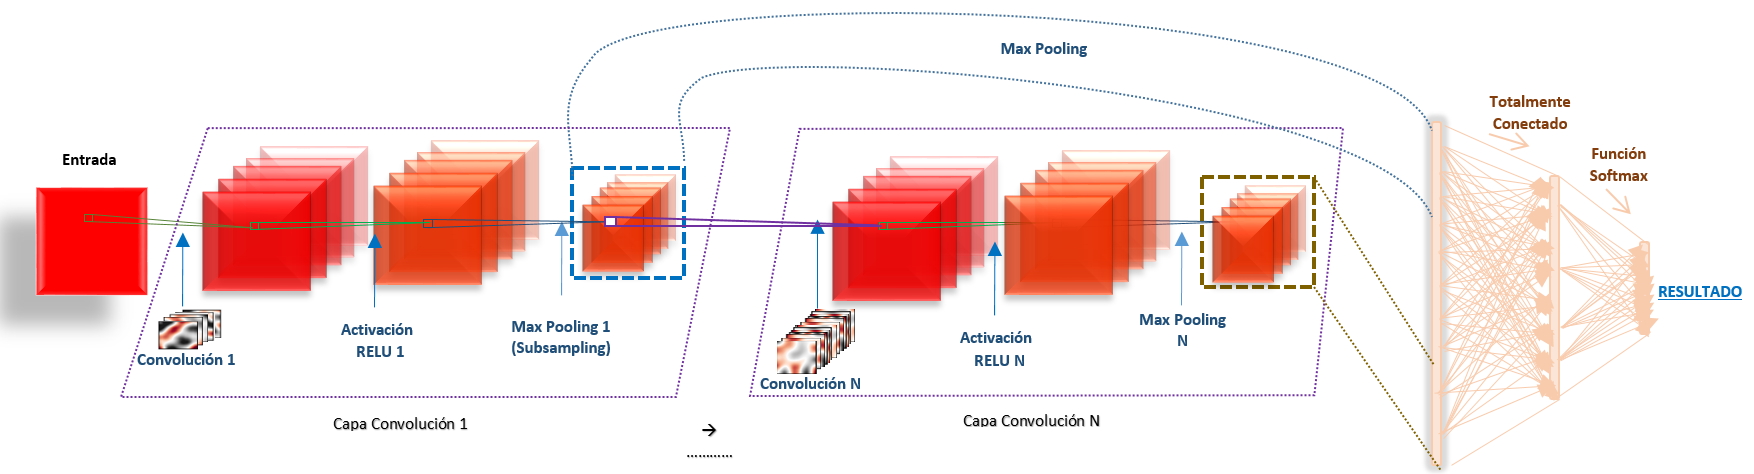
\includegraphics[width=1\textwidth]{images/desarrollo/networkArquitec/designNet}
		%\end{center}
		\begin{center}
		\caption{\small{Modelo del diseño de la Red propuesta}}
		{\small{\fontsize{10}{16.8}\selectfont {Fuente: Elaboración propia}}}
		\end{center}
		\vspace{-1.5em}
		\end{figure}

	Para el proceso de entrenamiento fueron tomados en cuenta 5 diferentes diseños. Estos fueron ejectudados durante el entrenamiento del dataset que contiene señales de tránsito de Alemania y Perú.

	Estos 5 modelos son descritos a continuación.
		\newpage 
		\subsubsection{Diseño A} 
			Diseño compuesto de 2 capas convolucionales y 2 capas totalmente conectadas.
			% Please add the following required packages to your document preamble:
			% \usepackage{multirow}
			% \usepackage[table,xcdraw]{xcolor}
			% If you use beamer only pass "xcolor=table" option, i.e. \documentclass[xcolor=table]{beamer}
			\begin{itemize}
			\item \underline{Dataset de Alemania}			
				\begin{table}[H]
				\begin{center}
				\caption{\small{Diseño A - Dataset de Imágenes de Alemania}}
				\begin{tabular}{|>{\scriptsize}c|>{\scriptsize}c>{\scriptsize}c>{\scriptsize}c>{\scriptsize}c>{\scriptsize}c|>{\scriptsize}c|}
				\hline
				{\color[HTML]{000000} \textbf{Capa}} & {\color[HTML]{000000} \textbf{Entrada}} & {\color[HTML]{000000} \textbf{Tipo}} & {\color[HTML]{000000} \textbf{\begin{tabular}[c]{@{}c@{}}Número de\\ (kernels/filtros)\end{tabular}}} & {\color[HTML]{000000} \textbf{Padding}} & {\textbf{Salida}} & {\textbf{Func.Esc.Múltiple}}\\ \hline

				 & 1 de 32 x 32 neuronas & Conv(DropOut : 0.8) & 32 de 3 x 3 & Activo & 32 de 32 x 32 neuronas & --\\ 
				\multirow{-2}{*}{1} &  32 de 32 x 32 neuronas &  Max Pool &  32 de 2 x 2 &  Inactivo & 32 de 16 x 16 neuronas & {\cellcolor[HTML]{DAE8FC}(Kernel = 2) 32 de 8x8}\\ \hline
				 & 32 de 16 x 16 neuronas & Conv(DropOut : 0.7) & 64 de 5 x 5 & Activo & 32 de 16 x 16 neuronas & --\\ 
				\multirow{-2}{*}{2} &  64 de 16 x 16 neuronas &  Max Pool &  64 de 2 x 2 &  Inactivo & 64 de 8 x 8 neuronas & {\cellcolor[HTML]{DAE8FC}(Kernel = 1) 64 de 8x8}\\ \hline
				3 &  {\cellcolor[HTML]{DAE8FC}6144 neuronas} &  F.C.(DropOut : 0.5) &  3072 neuronas &  -- & 43 neuronas & --\\ \hline

				\end{tabular}
				\end{center}
				\end{table}
			\vspace{-1.5em}
			\vskip 2cm
			\item \underline{Dataset del Perú}
				\begin{table}[H]
				\begin{center}
				\caption{\small{Diseño A - Dataset de Imágenes de Perú}}
				\begin{tabular}{|>{\scriptsize}c|>{\scriptsize}c>{\scriptsize}c>{\scriptsize}c>{\scriptsize}c>{\scriptsize}c|>{\scriptsize}c|}
				\hline
				{\color[HTML]{000000} \textbf{Capa}} & {\color[HTML]{000000} \textbf{Entrada}} & {\color[HTML]{000000} \textbf{Tipo}} & {\color[HTML]{000000} \textbf{\begin{tabular}[c]{@{}c@{}}Número de\\ (kernels/filtros)\end{tabular}}} & {\color[HTML]{000000} \textbf{Padding}} & {\textbf{Salida}} & {\textbf{Func.Esc.Múltiple}}\\ \hline

				 & 1 de 60 x 60 neuronas & Conv(DropOut : 0.8) & 32 de 3 x 3 & Activo & 32 de 60 x 60 neuronas & --\\ 
				\multirow{-2}{*}{1} &  32 de 60 x 60 neuronas &  Max Pool &  32 de 2 x 2 &  Inactivo & 32 de 30 x 30 neuronas & {\cellcolor[HTML]{DAE8FC}(Kernel = 2) 32 de 15x15}\\ \hline
				 & 32 de 30 x 30 neuronas & Conv(DropOut : 0.7) & 64 de 5 x 5 & Activo & 64 de 30 x 30 neuronas & --\\ 
				\multirow{-2}{*}{2} &  64 de 30 x 30 neuronas &  Max Pool &  64 de 2 x 2 &  Inactivo & 64 de 15 x 15 neuronas & {\cellcolor[HTML]{DAE8FC}(Kernel = 1) 64 de 15x15}\\ \hline
				3 &  {\cellcolor[HTML]{DAE8FC}21600 neuronas} &  F.C.(DropOut : 0.5) &  7200 neuronas &  -- & 7 neuronas & --\\ \hline

				\end{tabular}
				\end{center}
				\end{table}

			\end{itemize}
		%------------------------------------------------------------------------------------------------------------------------------------------------------------
		\vskip 2cm 
		\subsubsection{Diseño B}
		Diseño compuesto de 3 capas convolucionales y 2 capas totalmente conectadas.
			\begin{itemize}
			\item \underline{Dataset de Alemania}		
				\begin{table}[H]
				\begin{center}
				\caption{\small{Diseño B - Dataset de Imágenes de Alemania}}
				\begin{tabular}{|>{\scriptsize}c|>{\scriptsize}c>{\scriptsize}c>{\scriptsize}c>{\scriptsize}c>{\scriptsize}c|>{\scriptsize}c|}
				\hline
				{\color[HTML]{000000} \textbf{Capa}} & {\color[HTML]{000000} \textbf{Entrada}} & {\color[HTML]{000000} \textbf{Tipo}} & {\color[HTML]{000000} \textbf{\begin{tabular}[c]{@{}c@{}}Número de\\ (kernels/filtros)\end{tabular}}} & {\color[HTML]{000000} \textbf{Padding}} & {\textbf{Salida}} & {\textbf{Func.Esc.Múltiple}}\\ \hline

				 & 1 de 32 x 32 neuronas & Conv(DropOut : 0.8) & 32 de 3 x 3 & Activo & 32 de 32 x 32 neuronas & --\\ 
				\multirow{-2}{*}{1} &  32 de 32 x 32 neuronas &  Max Pool &  32 de 2 x 2 &  Inactivo & 32 de 16 x 16 neuronas & {\cellcolor[HTML]{DAE8FC}(Kernel = 4) 32 de 4x4}\\ \hline
				 & 32 de 16 x 16 neuronas & Conv(DropOut : 0.7) & 64 de 5 x 5 & Activo & 64 de 16 x 16 neuronas & --\\ 
				\multirow{-2}{*}{2} &  64 de 16 x 16 neuronas &  Max Pool &  64 de 2 x 2 &  Inactivo & 64 de 8 x 8 neuronas & {\cellcolor[HTML]{DAE8FC}(Kernel = 2) 64 de 4x4}\\ \hline			
				{\cellcolor[HTML]{ffb3b3}} & 64 de 8 x 8 neuronas & Conv(DropOut : 0.6) & 128 de 5 x 5 & Activo & 128 de 8 x 8 neuronas & --\\ 			
				{\cellcolor[HTML]{ffb3b3} \multirow{-2}{*}{3}} &  128 de 8 x 8 neuronas &  Max Pool &  128 de 2 x 2 &  Inactivo & 128 de 4 x 4 neuronas & {\cellcolor[HTML]{DAE8FC} (Kernel = 1) 128 de 4x4 }\\ \hline
				4 &  {\cellcolor[HTML]{DAE8FC}3584 neuronas} &  F.C.(DropOut : 0.5) &  1024 neuronas &  -- & 43 neuronas & --\\ \hline
				\end{tabular}
				\end{center}
				\end{table}
			\vspace{2em}
			%\vskip 2cm
			\item \underline{Dataset del Perú}
				\begin{table}[H]
				\begin{center}
				\caption{\small{Diseño B - Dataset de Imágenes de Perú}}
				\begin{tabular}{|>{\scriptsize}c|>{\scriptsize}c>{\scriptsize}c>{\scriptsize}c>{\scriptsize}c>{\scriptsize}c|>{\scriptsize}c|}
				\hline
				{\color[HTML]{000000} \textbf{Capa}} & {\color[HTML]{000000} \textbf{Entrada}} & {\color[HTML]{000000} \textbf{Tipo}} & {\color[HTML]{000000} \textbf{\begin{tabular}[c]{@{}c@{}}Número de\\ (kernels/filtros)\end{tabular}}} & {\color[HTML]{000000} \textbf{Padding}} & {\textbf{Salida}} & {\textbf{Func.Esc.Múltiple}}\\ \hline

				 & 1 de 60 x 60 neuronas & Conv(DropOut : 0.8) & 32 de 3 x 3 & Activo & 32 de 60 x 60 neuronas & --\\ 
				\multirow{-2}{*}{1} &  32 de 60 x 60 neuronas &  Max Pool &  32 de 2 x 2 &  Inactivo & 32 de 30 x 30 neuronas & {\cellcolor[HTML]{DAE8FC}(Kernel = 4) 32 de 7x7}\\ \hline
				 & 32 de 30 x 30 neuronas & Conv(DropOut : 0.7) & 64 de 5 x 5 & Activo & 64 de 30 x 30 neuronas & --\\ 
				\multirow{-2}{*}{2} &  64 de 30 x 30 neuronas &  Max Pool &  64 de 2 x 2 &  Inactivo & 64 de 15 x 15 neuronas & {\cellcolor[HTML]{DAE8FC}(Kernel = 2) 64 de 7x7}\\ \hline			
				{\cellcolor[HTML]{ffb3b3}} & 64 de 15 x 15 neuronas & Conv(DropOut : 0.6) & 128 de 5 x 5 & Activo & 128 de 15 x 15 neuronas & --\\ 			
				{\cellcolor[HTML]{ffb3b3} \multirow{-2}{*}{3}} &  128 de 15 x 15 neuronas &  Max Pool &  128 de 2 x 2 &  Inactivo & 128 de 7 x 7 neuronas & {\cellcolor[HTML]{DAE8FC} (Kernel = 1) 128 de 7x7 }\\ \hline
				4 &  {\cellcolor[HTML]{DAE8FC}10976 neuronas} &  F.C.(DropOut : 0.5) &  2700 neuronas &  -- & 7 neuronas & --\\ \hline
				\end{tabular}
				\end{center}
				\end{table}

				\end{itemize}
		%------------------------------------------------------------------------------------------------------------------------------------------------------------
		\vspace{2.2em}
		\subsubsection{Diseño C} %model4
			\vspace{-1.2em}
			Diseño compuesto de 3 capas convolucionales y 2 capas totalmente conectadas. Variando el número de kernels en la 2da capa convolucional.
			
			\begin{itemize}
			\item \underline{Dataset de Alemania}		
				\begin{table}[H]
				\begin{center}
				\caption{\small{Diseño C - Dataset de Imágenes de Alemania}}
				\begin{tabular}{|>{\scriptsize}c|>{\scriptsize}c>{\scriptsize}c>{\scriptsize}c>{\scriptsize}c>{\scriptsize}c|>{\scriptsize}c|}
				\hline
				{\color[HTML]{000000} \textbf{Capa}} & {\color[HTML]{000000} \textbf{Entrada}} & {\color[HTML]{000000} \textbf{Tipo}} & {\color[HTML]{000000} \textbf{\begin{tabular}[c]{@{}c@{}}Número de\\ (kernels/filtros)\end{tabular}}} & {\color[HTML]{000000} \textbf{Padding}} & {\textbf{Salida}} & {\textbf{Func.Esc.Múltiple}}\\ \hline

				 & 1 de 32 x 32 neuronas & Conv(DropOut : 0.8) & 32 de 3 x 3 & Activo & 32 de 32 x 32 neuronas & --\\ 
				\multirow{-2}{*}{1} &  32 de 32 x 32 neuronas &  Max Pool &  32 de 2 x 2 &  Inactivo & 32 de 16 x 16 neuronas & {\cellcolor[HTML]{DAE8FC}(Kernel = 4) 32 de 4x4}\\ \hline
				 & 32 de 16 x 16 neuronas & Conv(DropOut : 0.7) & {\cellcolor[HTML]{ffb3b3} 64 de 3 x 3} & Activo & 64 de 16 x 16 neuronas & --\\ 
				\multirow{-2}{*}{2} &  64 de 16 x 16 neuronas &  Max Pool &  64 de 2 x 2 &  Inactivo & 64 de 8 x 8 neuronas & {\cellcolor[HTML]{DAE8FC}(Kernel = 2) 64 de 4x4}\\ \hline			
				 & 64 de 8 x 8 neuronas & Conv(DropOut : 0.6) & 128 de 5 x 5 & Activo & 64 de 8 x 8 neuronas & --\\ 			
				\multirow{-2}{*}{3} &  128 de 8 x 8 neuronas &  Max Pool &  128 de 2 x 2 &  Inactivo & 128 de 4 x 4 neuronas & {\cellcolor[HTML]{DAE8FC} (Kernel = 1) 128 de 4x4 }\\ \hline
				4 &  {\cellcolor[HTML]{DAE8FC}3584 neuronas} &  F.C.(DropOut : 0.5) &  1024 neuronas &  -- & 43 neuronas & --\\ \hline
				\end{tabular}
				\end{center}
				\end{table}
			\vspace{-1.5em}
			%\vskip 2cm
			\item \underline{Dataset del Perú}
				\begin{table}[H]
				\begin{center}
				\caption{\small{Diseño C - Dataset de Imágenes de Perú}}
				\begin{tabular}{|>{\scriptsize}c|>{\scriptsize}c>{\scriptsize}c>{\scriptsize}c>{\scriptsize}c>{\scriptsize}c|>{\scriptsize}c|}
				\hline
				{\color[HTML]{000000} \textbf{Capa}} & {\color[HTML]{000000} \textbf{Entrada}} & {\color[HTML]{000000} \textbf{Tipo}} & {\color[HTML]{000000} \textbf{\begin{tabular}[c]{@{}c@{}}Número de\\ (kernels/filtros)\end{tabular}}} & {\color[HTML]{000000} \textbf{Padding}} & {\textbf{Salida}} & {\textbf{Func.Esc.Múltiple}}\\ \hline

				 & 1 de 60 x 60 neuronas & Conv(DropOut : 0.8) & 32 de 3 x 3 & Activo & 32 de 60 x 60 neuronas & --\\ 
				\multirow{-2}{*}{1} &  32 de 60 x 60 neuronas &  Max Pool &  32 de 2 x 2 &  Inactivo & 32 de 30 x 30 neuronas & {\cellcolor[HTML]{DAE8FC}(Kernel = 4) 32 de 7x7}\\ \hline
				 & 32 de 30 x 30 neuronas & Conv(DropOut : 0.7) & {\cellcolor[HTML]{ffb3b3} 64 de 3 x 3} & Activo & 64 de 30 x 30 neuronas & --\\ 
				\multirow{-2}{*}{2} &  64 de 30 x 30 neuronas &  Max Pool &  64 de 2 x 2 &  Inactivo & 64 de 15 x 15 neuronas & {\cellcolor[HTML]{DAE8FC}(Kernel = 2) 64 de 7x7}\\ \hline			
				 & 64 de 15 x 15 neuronas & Conv(DropOut : 0.6) & 128 de 5 x 5 & Activo & 128 de 15 x 15 neuronas & --\\ 			
				\multirow{-2}{*}{3} &  128 de 15 x 15 neuronas &  Max Pool &  128 de 2 x 2 &  Inactivo & 128 de 7 x 7 neuronas & {\cellcolor[HTML]{DAE8FC} (Kernel = 1) 128 de 7x7 }\\ \hline
				4 &  {\cellcolor[HTML]{DAE8FC}10976 neuronas} &  F.C.(DropOut : 0.5) &  2700 neuronas &  -- & 7 neuronas & --\\ \hline
				\end{tabular}
				\end{center}
				\end{table}

			\end{itemize}
		%------------------------------------------------------------------------------------------------------------------------------------------------------------

		\subsubsection{Diseño D} %model6
			
			Diseño compuesto de 3 capas convolucionales y 2 capas totalmente conectadas. Variando el número de kernels en la 3ra capa convolucional.

			\begin{itemize}
			\item \underline{Dataset de Alemania}		

				\begin{table}[H]
				\begin{center}
				\caption{\small{Diseño D - Dataset de Imágenes de Alemania}}
				\begin{tabular}{|>{\scriptsize}c|>{\scriptsize}c>{\scriptsize}c>{\scriptsize}c>{\scriptsize}c>{\scriptsize}c|>{\scriptsize}c|}
				\hline
				{\color[HTML]{000000} \textbf{Capa}} & {\color[HTML]{000000} \textbf{Entrada}} & {\color[HTML]{000000} \textbf{Tipo}} & {\color[HTML]{000000} \textbf{\begin{tabular}[c]{@{}c@{}}Número de\\ (kernels/filtros)\end{tabular}}} & {\color[HTML]{000000} \textbf{Padding}} & {\textbf{Salida}} & {\textbf{Func.Esc.Múltiple}}\\ \hline

				 & 1 de 32 x 32 neuronas & Conv(DropOut : 0.8) & 32 de 3 x 3 & Activo & 32 de 32 x 32 neuronas & --\\ 
				\multirow{-2}{*}{1} &  32 de 32 x 32 neuronas &  Max Pool &  32 de 2 x 2 &  Inactivo & 32 de 16 x 16 neuronas & {\cellcolor[HTML]{DAE8FC}(Kernel = 4) 32 de 4x4}\\ \hline
				 & 32 de 16 x 16 neuronas & Conv(DropOut : 0.7) & 64 de 5 x 5 & Activo & 64 de 16 x 16 neuronas & --\\ 
				\multirow{-2}{*}{2} &  64 de 16 x 16 neuronas &  Max Pool &  64 de 2 x 2 &  Inactivo & 64 de 8 x 8 neuronas & {\cellcolor[HTML]{DAE8FC}(Kernel = 2) 64 de 4x4}\\ \hline			
				 & 64 de 8 x 8 neuronas & Conv(DropOut : 0.6) & {\cellcolor[HTML]{ffb3b3} 128 de 7 x 7} & Activo & 64 de 8 x 8 neuronas & --\\ 			
				\multirow{-2}{*}{3} &  128 de 8 x 8 neuronas &  Max Pool &  128 de 2 x 2 &  Inactivo & 128 de 4 x 4 neuronas & {\cellcolor[HTML]{DAE8FC} (Kernel = 1) 128 de 4x4 }\\ \hline
				4 &  {\cellcolor[HTML]{DAE8FC}3584 neuronas} &  F.C.(DropOut : 0.5) &  1024 neuronas &  -- & 43 neuronas & --\\ \hline
				\end{tabular}
				\end{center}
				\end{table}

			\item \underline{Dataset del Perú}
				\begin{table}[H]
				\begin{center}
				\caption{\small{Diseño D - Dataset de Imágenes de Perú}}
				\begin{tabular}{|>{\scriptsize}c|>{\scriptsize}c>{\scriptsize}c>{\scriptsize}c>{\scriptsize}c>{\scriptsize}c|>{\scriptsize}c|}
				\hline
				{\color[HTML]{000000} \textbf{Capa}} & {\color[HTML]{000000} \textbf{Entrada}} & {\color[HTML]{000000} \textbf{Tipo}} & {\color[HTML]{000000} \textbf{\begin{tabular}[c]{@{}c@{}}Número de\\ (kernels/filtros)\end{tabular}}} & {\color[HTML]{000000} \textbf{Padding}} & {\textbf{Salida}} & {\textbf{Func.Esc.Múltiple}}\\ \hline

				 & 1 de 60 x 60 neuronas & Conv(DropOut : 0.8) & 32 de 3 x 3 & Activo & 32 de 60 x 60 neuronas & --\\ 
				\multirow{-2}{*}{1} &  32 de 60 x 60 neuronas &  Max Pool &  32 de 2 x 2 &  Inactivo & 32 de 30 x 30 neuronas & {\cellcolor[HTML]{DAE8FC}(Kernel = 4) 32 de 7x7}\\ \hline
				 & 32 de 30 x 30 neuronas & Conv(DropOut : 0.7) & 64 de 5 x 5 & Activo & 64 de 30 x 30 neuronas & --\\ 
				\multirow{-2}{*}{2} &  64 de 30 x 30 neuronas &  Max Pool &  64 de 2 x 2 &  Inactivo & 64 de 15 x 15 neuronas & {\cellcolor[HTML]{DAE8FC}(Kernel = 2) 64 de 7x7}\\ \hline			
				 & 64 de 15 x 15 neuronas & Conv(DropOut : 0.6) & {\cellcolor[HTML]{ffb3b3} 128 de 7 x 7} & Activo & 128 de 15 x 15 neuronas & --\\ 			
				\multirow{-2}{*}{3} &  128 de 15 x 15 neuronas &  Max Pool &  128 de 2 x 2 &  Inactivo & 128 de 7 x 7 neuronas & {\cellcolor[HTML]{DAE8FC} (Kernel = 1) 128 de 7x7 }\\ \hline
				4 &  {\cellcolor[HTML]{DAE8FC}10976 neuronas} &  F.C.(DropOut : 0.5) &  2700 neuronas &  -- & 7 neuronas & --\\ \hline
				\end{tabular}
				\end{center}
				\end{table}

			\end{itemize}
		%------------------------------------------------------------------------------------------------------------------------------------------------------------
		%\newpage
		\subsubsection{Diseño E}
			Diseño compuesto de 4 capas convolucionales y 2 capas totalmente conectadas.
			\begin{itemize}
			\item \underline{Dataset de Alemania}		

				\begin{table}[H]
				\begin{center}
				\caption{\small{Diseño E - Dataset de Imágenes de Alemania}}
				\begin{tabular}{|>{\scriptsize}c|>{\scriptsize}c>{\scriptsize}c>{\scriptsize}c>{\scriptsize}c>{\scriptsize}c|>{\scriptsize}c|}
				\hline
				{\color[HTML]{000000} \textbf{Capa}} & {\color[HTML]{000000} \textbf{Entrada}} & {\color[HTML]{000000} \textbf{Tipo}} & {\color[HTML]{000000} \textbf{\begin{tabular}[c]{@{}c@{}}Número de\\ (kernels/filtros)\end{tabular}}} & {\color[HTML]{000000} \textbf{Padding}} & {\textbf{Salida}} & {\textbf{Func.Esc.Múltiple}}\\ \hline

				 & 1 de 32 x 32 neuronas & Conv(DropOut : 0.8) & 32 de 3 x 3 & Activo & 32 de 32 x 32 neuronas & --\\ 
				\multirow{-2}{*}{1} &  32 de 32 x 32 neuronas &  Max Pool &  32 de 2 x 2 &  Inactivo & 32 de 16 x 16 neuronas & {\cellcolor[HTML]{DAE8FC}(Kernel = 8) 32 de 2x2}\\ \hline
				 & 32 de 16 x 16 neuronas & Conv(DropOut : 0.7) & 64 de 5 x 5 & Activo & 64 de 16 x 16 neuronas & --\\ 
				\multirow{-2}{*}{2} &  64 de 16 x 16 neuronas &  Max Pool &  64 de 2 x 2 &  Inactivo & 64 de 8 x 8 neuronas & {\cellcolor[HTML]{DAE8FC}(Kernel = 4) 64 de 2x2}\\ \hline			
				 & 64 de 8 x 8 neuronas & Conv(DropOut : 0.6) & 128 de 5 x 5 & Activo & 128 de 8 x 8 neuronas & --\\ 			
				\multirow{-2}{*}{3} &  128 de 8 x 8 neuronas &  Max Pool &  128 de 2 x 2 &  Inactivo & 128 de 4 x 4 neuronas & {\cellcolor[HTML]{DAE8FC} (Kernel = 2) 128 de 2x2 }\\ \hline
				{\cellcolor[HTML]{ffb3b3}}& 128 de 4 x 4 neuronas & Conv(DropOut : 0.6) & 128 de 7 x 7 & Activo & 128 de 4 x 4 neuronas & --\\ 			
				{\cellcolor[HTML]{ffb3b3}\multirow{-2}{*}{4}} &  128 de 4 x 4 neuronas &  Max Pool &  128 de 2 x 2 &  Inactivo & 128 de 2 x 2 neuronas & {\cellcolor[HTML]{DAE8FC} (Kernel = 1) 128 de 2x2 }\\ \hline
				5 &  {\cellcolor[HTML]{DAE8FC}1408 neuronas} &  F.C.(DropOut : 0.5) &  702 neuronas &  -- & 43 neuronas & --\\ \hline
				\end{tabular}
				\end{center}
				\end{table}

			\vspace{-1.5em}
			
			\item \underline{Dataset del Perú}

				\begin{table}[H]
				\begin{center}
				\caption{\small{Diseño E - Dataset de Imágenes de Perú}}
				\begin{tabular}{|>{\scriptsize}c|>{\scriptsize}c>{\scriptsize}c>{\scriptsize}c>{\scriptsize}c>{\scriptsize}c|>{\scriptsize}c|}
				\hline
				{\color[HTML]{000000} \textbf{Capa}} & {\color[HTML]{000000} \textbf{Entrada}} & {\color[HTML]{000000} \textbf{Tipo}} & {\color[HTML]{000000} \textbf{\begin{tabular}[c]{@{}c@{}}Número de\\ (kernels/filtros)\end{tabular}}} & {\color[HTML]{000000} \textbf{Padding}} & {\textbf{Salida}} & {\textbf{Func.Esc.Múltiple}}\\ \hline

				 & 1 de 60 x 60 neuronas & Conv(DropOut : 0.8) & 32 de 3 x 3 & Activo & 32 de 60 x 60 neuronas & --\\ 
				\multirow{-2}{*}{1} &  32 de 60 x 60 neuronas &  Max Pool &  32 de 2 x 2 &  Inactivo & 32 de 30 x 30 neuronas & {\cellcolor[HTML]{DAE8FC}(Kernel = 8) 32 de 3x3}\\ \hline
				 & 32 de 30 x 30 neuronas & Conv(DropOut : 0.7) & 64 de 5 x 5 & Activo & 64 de 30 x 30 neuronas & --\\ 
				\multirow{-2}{*}{2} &  64 de 30 x 30 neuronas &  Max Pool &  64 de 2 x 2 &  Inactivo & 64 de 15 x 15 neuronas & {\cellcolor[HTML]{DAE8FC}(Kernel = 4) 64 de 3x3}\\ \hline			
				 & 64 de 15 x 15 neuronas & Conv(DropOut : 0.6) & 128 de 5 x 5 & Activo & 128 de 15 x 15 neuronas & --\\ 			
				\multirow{-2}{*}{3} &  128 de 15 x 15 neuronas &  Max Pool &  128 de 2 x 2 &  Inactivo & 128 de 7 x 7 neuronas & {\cellcolor[HTML]{DAE8FC} (Kernel = 2) 128 de 3x3 }\\ \hline
				{\cellcolor[HTML]{ffb3b3}}& 128 de 7 x 7 neuronas & Conv(DropOut : 0.6) & 128 de 7 x 7 & Activo & 128 de 7 x 7 neuronas & --\\ 			
				{\cellcolor[HTML]{ffb3b3}\multirow{-2}{*}{4}} &  128 de 7 x 7 neuronas &  Max Pool &  128 de 2 x 2 &  Inactivo & 128 de 3 x 3 neuronas & {\cellcolor[HTML]{DAE8FC} (Kernel = 1) 128 de 3x3 }\\ \hline
				5 &  {\cellcolor[HTML]{DAE8FC}3168 neuronas} &  F.C.(DropOut : 0.5) &  1584 neuronas &  -- & 7 neuronas & --\\ \hline
				\end{tabular}
				\end{center}
				\end{table}

			\end{itemize}

			En el apéndice A se muestran bloques de pseudocódigo que fueron implementados para la construcción de los diseños de Red.
		%------------------------------------------------------------------------------------------------------------------------------------------------------------
%\newpage
\section{Entrenamiento y Validación }

	Para estimar el error de clasificación, como fue mencionado en la \textbf{Seccion 2.3}, se utilizó el méto do de validación cruzada. En la estimación del error se usa el conjunto de muestras disponible, el cual se divide en el conjunto de entrenamiento y el de validación. El clasificador se diseña usando las muestras de entrenamiento y luego se evalúa obteniendo el error de clasificación para las muestras de validación. Con base en el error obtenido se puede predecir el desempeño del clasificador ante nuevas muestras. Para obtener una medida confiable del desempeño, el conjunto de muestras es lo suficientemente grande y los conjuntos de entrenamiento y de validación son independientes.


	\subsection{Señales de Tránsito de Alemania}

		Luego de haber entrenado las diferentes arquitecturas durante 100 épocas(38700 iteraciones), obtenemos los siguientes resultados:
		%------------------------------------------------------------------------------------------------------------------------------------------------------------
	 	\subsubsection{Análisis del Entrenamiento y Validación del Diseño A}  
			\begin{figure}[H]
				\begin{center}
				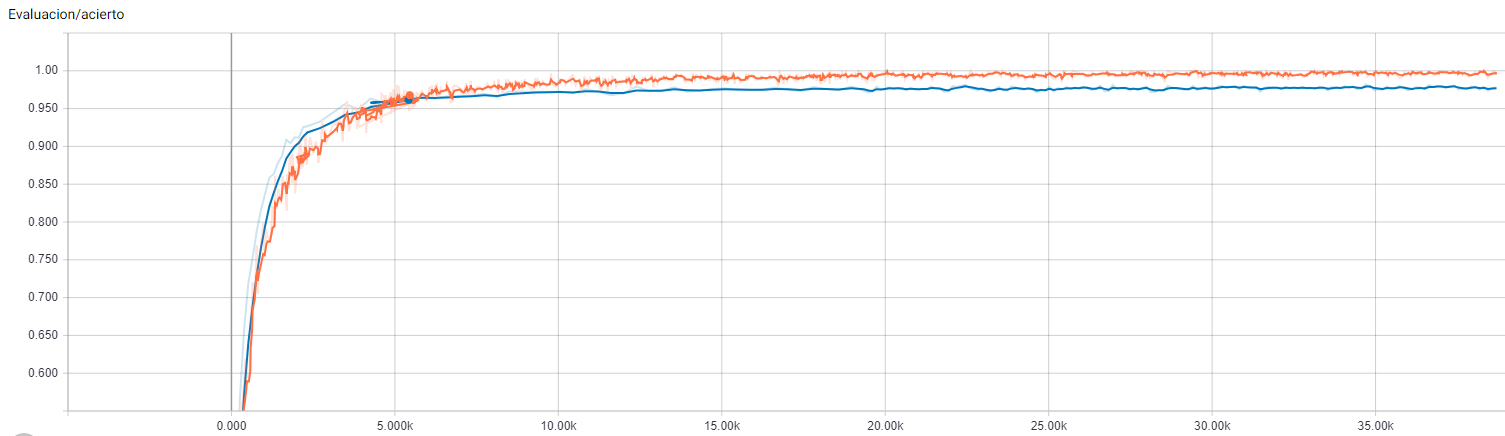
\includegraphics[width=1\textwidth]{images/desarrollo/trainResults/german/model0Acierto} 
				\end{center}
				\begin{center}
				\caption{\small{Modelo A Tasa de Acierto por iteración - Dataset de imágenes de Alemania  }}
				
				{\small{\fontsize{10}{16.8}\selectfont {Fuente: Elaboración propia}}}
				\end{center}
				\vspace{-1.5em}
			\end{figure}

			\begin{figure}[H]
				\begin{center}
				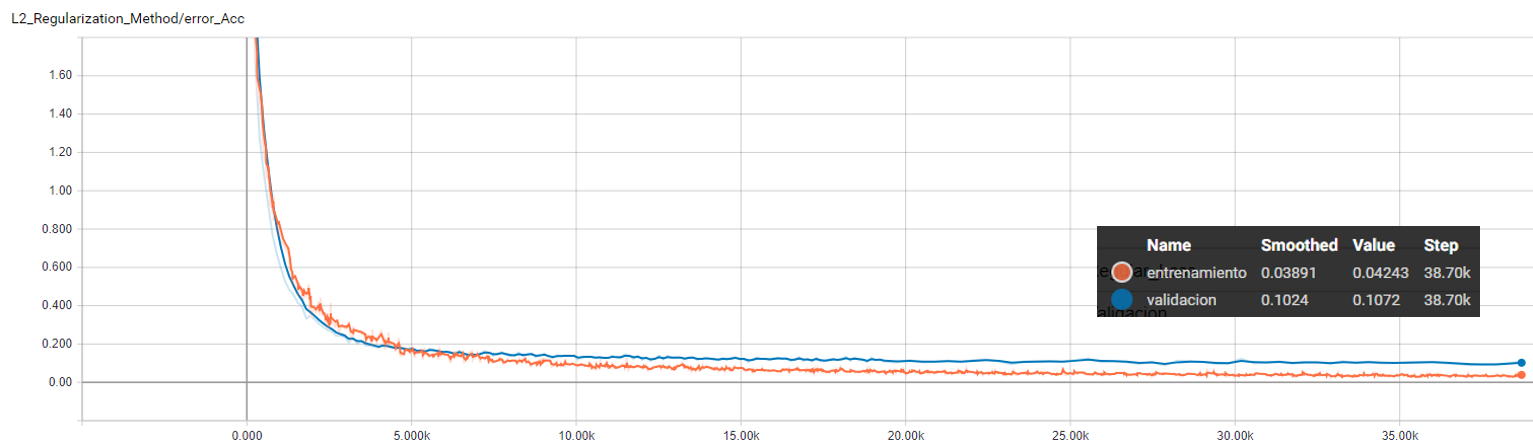
\includegraphics[width=1\textwidth]{images/desarrollo/trainResults/german/model0Loss_1} 
				\end{center}
				\begin{center}
				\caption{\small{Modelo A Tasa de pérdida por iteración - Dataset de imágenes de Alemania}}
				
				{\small{\fontsize{10}{16.8}\selectfont {Fuente: Elaboración propia}}}
				\end{center}
				\vspace{-1.5em}
			\end{figure}

			Luego de 20 épocas iteradas(aproximadamente  7000 iteraciones), se observa que rápidamente el modelo se sobreajusta al dataset de entrenamiento. Es decir, rápidamente el valor de pérdida es muy cercana a cero, lo que a su vez hace que se separe de manera abrupta de los resultados de validación y lo mismo sucede con la tase de acierto, en la cual la de validación luego de estas 20 épocas es mucho menor al de entrenamiento. Iteraciones posteriores no permitirán mejores resultados.


		%------------------------------------------------------------------------------------------------------------------------------------------------------------
		\subsubsection{Análisis del Entrenamiento y Validación del Diseño B}  
		
			\begin{figure}[H]
				\begin{center}
				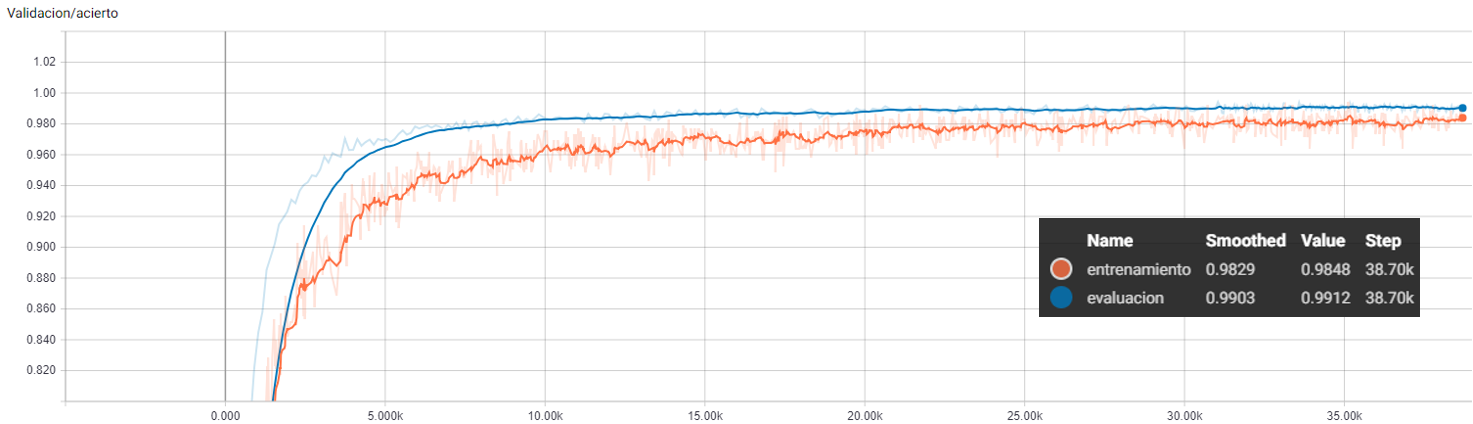
\includegraphics[width=1\textwidth]{images/desarrollo/trainResults/german/model1Acierto} 
				\end{center}
				\begin{center}
				\caption{\small{Modelo B Tasa de Acierto por iteración - Dataset de imágenes de Alemania  }}
				
				{\small{\fontsize{10}{16.8}\selectfont {Fuente: Elaboración propia}}}
				\end{center}
				\vspace{-1.5em}
			\end{figure}
		
			
			\begin{figure}[H]
				\begin{center}
				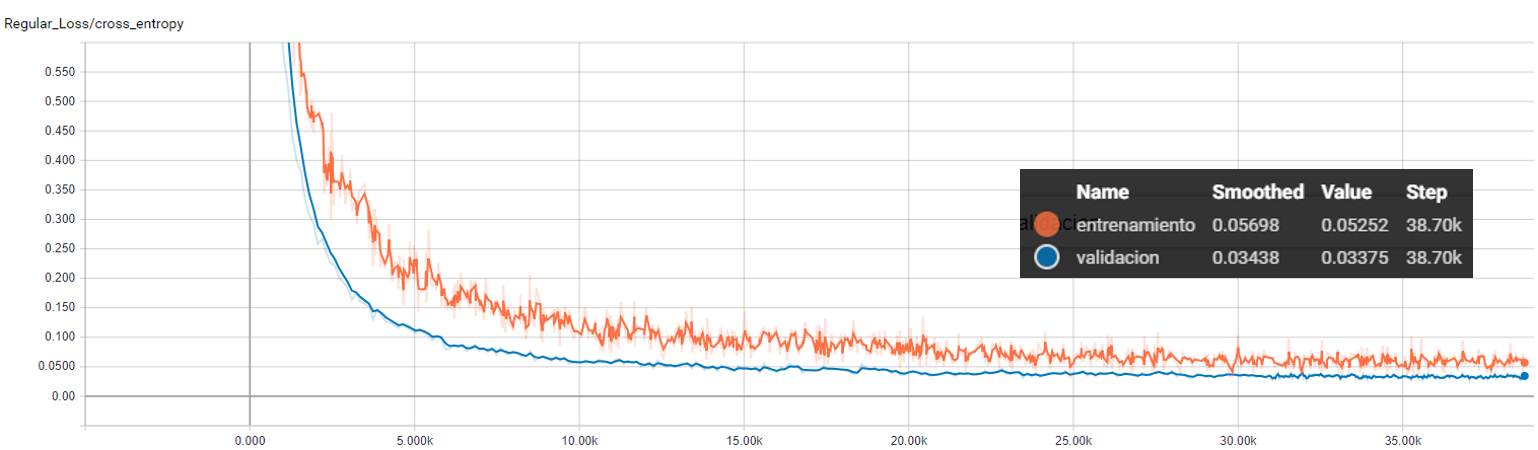
\includegraphics[width=1\textwidth]{images/desarrollo/trainResults/german/model1Loss_1} 
				\end{center}
				\begin{center}
				\caption{\small{Modelo B Tasa de pérdida por iteración - Dataset de imágenes de Alemania}}
				
				{\small{\fontsize{10}{16.8}\selectfont {Fuente: Elaboración propia}}}
				\end{center}
				\vspace{-1.5em}
			\end{figure}

			Durante 100 épocas iteradas(38700 iteraciones), apartir de \textbf{34830 iteraciones(80 épocas)} se obtiene la mejor tasa de acierto de validación(99.12\%) logrando resultados muy similares entre la tasa de acierto y pérdida del entrenamiento y validación, por lo que iteraciones posteriores harán que el modelo se sobreajuste al conjunto de entrenamiento y no permita evaluar correctamente imágenes previamente no analizadas.


		%------------------------------------------------------------------------------------------------------------------------------------------------------------

		\subsubsection{Análisis del Entrenamiento y Validación del Diseño C} 

			\begin{figure}[H]
				\begin{center}
				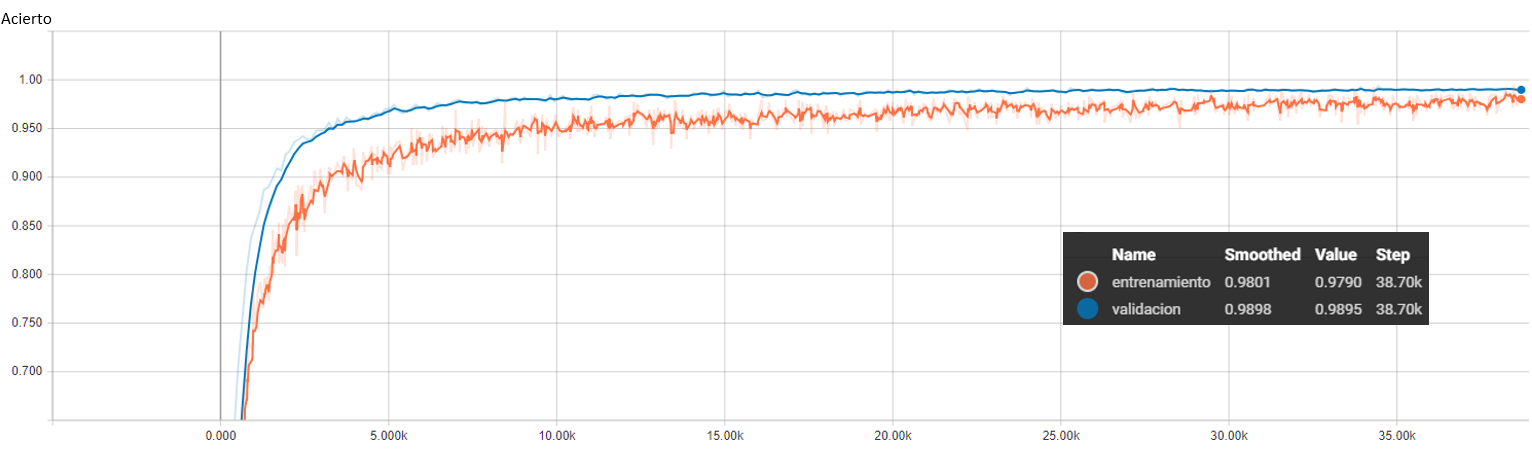
\includegraphics[width=1\textwidth]{images/desarrollo/trainResults/german/model4Acierto} 
				\end{center}
				\begin{center}
				\caption{\small{Modelo C Tasa de Acierto por iteración - Dataset de imágenes de Alemania  }}
				
				{\small{\fontsize{10}{16.8}\selectfont {Fuente: Elaboración propia}}}
				\end{center}
				\vspace{-1.5em}
			\end{figure}
			
			
			\begin{figure}[H]
				\begin{center}
				\includegraphics[width=1\textwidth]{images/desarrollo/trainResults/german/model4Loss_1} 
				\end{center}
				\begin{center}
				\caption{\small{Modelo C Tasa de pérdida por iteración - Dataset de imágenes de Alemania}}
				
				{\small{\fontsize{10}{16.8}\selectfont {Fuente: Elaboración propia}}}
				\end{center}
				\vspace{-1.5em}
			\end{figure}

			Al igual que el modelo anterior, luego de 100 épocas iteradas(38700 iteraciones), se obtiene la mejor tasa de acierto y pérdida en la validación logrando resultados muy similares entre el entrenamiento y la validación, por lo que iteraciones posteriores harán que el modelo se sobreajuste al conjunto de entrenamiento y no permita evaluar correctamente imágenes previamente no analizadas.


		%------------------------------------------------------------------------------------------------------------------------------------------------------------			
		\subsubsection{Análisis del Entrenamiento y Validación del Diseño D} 
			\begin{figure}[H]
				\begin{center}
				\includegraphics[width=1\textwidth]{images/desarrollo/trainResults/german/model6Acierto} 
				\end{center}
				\begin{center}
				\caption{\small{Modelo D Tasa de Acierto por iteración - Dataset de imágenes de Alemania  }}
				
				{\small{\fontsize{10}{16.8}\selectfont {Fuente: Elaboración propia}}}
				\end{center}
				\vspace{-1.5em}
			\end{figure}
			
			\begin{figure}[H]
				\begin{center}
				\includegraphics[width=1\textwidth]{images/desarrollo/trainResults/german/model6Loss_1} 
				\end{center}
				\begin{center}
				\caption{\small{Modelo D Tasa de pérdida por iteración - Dataset de imágenes de Alemania}}
				
				{\small{\fontsize{10}{16.8}\selectfont {Fuente: Elaboración propia}}}
				\end{center}
				\vspace{-1.5em}
			\end{figure}

			Al finalizar 100 épocas (38700 iteraciones) se obtiene la mejor de las tasas de acierto y pérdida en la validación. Iteraciones posteriores harán probablemente que el modelo se sobreajuste al conjunto de entrenamiento y no permita evaluar correctamente imágenes previamente no analizadas.
			

		%------------------------------------------------------------------------------------------------------------------------------------------------------------
		\subsubsection{Análisis del Entrenamiento y Validación del Diseño E} 
			\begin{figure}[H]
				\begin{center}
				\includegraphics[width=1\textwidth]{images/desarrollo/trainResults/german/model7Acierto} 
				\end{center}
				\begin{center}
				\caption{\small{Modelo E Tasa de Acierto por iteración - Dataset de imágenes de Alemania  }}
				
				{\small{\fontsize{10}{16.8}\selectfont {Fuente: Elaboración propia}}}
				\end{center}
				\vspace{-1.5em}
			\end{figure}
		
			\begin{figure}[H]
				\begin{center}
				\includegraphics[width=1\textwidth]{images/desarrollo/trainResults/german/model7Loss_1} 
				\end{center}
				\begin{center}
				\caption{\small{Modelo E Tasa de pérdida por iteración - Dataset de imágenes de Alemania}}
				
				{\small{\fontsize{10}{16.8}\selectfont {Fuente: Elaboración propia}}}
				\end{center}
				\vspace{-1.5em}
			\end{figure}
		
			Poco antes de finalizar las 100 épocas (38700 iteraciones) se obtiene una de las mejores tasas de acierto de validación y una de las tasas más mínimas de pérdida (error).
		%------------------------------------------------------------------------------------------------------------------------------------------------------------
		
		\vspace{2em}
		En resumen, los 5 modelos lograron similares resultados de acierto y error durante el entrenamiento.

			\begin{figure}[H]
				%\begin{center}
				\includegraphics[width=1\textwidth, height=\textheight,keepaspectratio]{images/desarrollo/trainResults/germanSummary_entreAcierto} 
				%\end{center}
				\begin{center}
				\caption{\small{Análisis del Acierto durante el Entrenamiento de los modelos - Dataset Señales de Tránsito de Alemania}}
				
				{\small{\fontsize{10}{16.8}\selectfont {Fuente: Elaboración propia}}}
				\end{center}
				\vspace{-1.5em}
			\end{figure}	

			\begin{figure}[H]
				%\begin{center}
				\includegraphics[width=1\textwidth, height=\textheight,keepaspectratio]{images/desarrollo/trainResults/germanSummary_entreError} 
				%\end{center}
				\begin{center}
				\caption{\small{Análisis del Error durante el Entrenamiento de los modelos - Dataset Señales de Tránsito de Alemania}}
				
				{\small{\fontsize{10}{16.8}\selectfont {Fuente: Elaboración propia}}}
				\end{center}
				\vspace{-1.5em}
			\end{figure}	


			Sin embargo a través de la validación del modelo (usando dataset de imágenes no visto/analizado durante el entrenamiento), se puede apreciar que el Modelo E obtuvo una de las mejores tasas de Acierto y Error. 

			\begin{figure}[H]
				%\begin{center}
				\includegraphics[width=1\textwidth, height=\textheight,keepaspectratio]{images/desarrollo/trainResults/germanSummary_validAcierto} 
				%\end{center}
				\begin{center}
				\caption{\small{Análisis del Acierto en la Validación de los modelos - Dataset Señales de Tránsito de Alemania}}
				
				{\small{\fontsize{10}{16.8}\selectfont {Fuente: Elaboración propia}}}
				\end{center}
				\vspace{-1.5em}
			\end{figure}

			\begin{figure}[H]
				%\begin{center}
				\includegraphics[width=1\textwidth, height=\textheight,keepaspectratio]{images/desarrollo/trainResults/germanSummary_validError} 
				%\end{center}
				\begin{center}
				\caption{\small{Análisis del Error en la Validación de los modelos - Dataset Señales de Tránsito de Alemania}}
				
				{\small{\fontsize{10}{16.8}\selectfont {Fuente: Elaboración propia}}}
				\end{center}
				\vspace{-1.5em}
			\end{figure}
	









	\newpage
	\subsection{Señales de Tránsito de Perú}
		Luego de haber entrenado las diferentes arquitecturas durante 100 épocas (7700 iteraciones), obtenemos los siguientes resultados:

		\subsubsection{Análisis del Entrenamiento y Validación del Diseño A}  
			\begin{figure}[H]
				\begin{center}
				\includegraphics[width=1\textwidth]{images/desarrollo/trainResults/peru/model0Acierto} 
				\end{center}
				\begin{center}
				\caption{\small{Modelo A Tasa de Acierto por iteración - Dataset de imágenes de Perú  }}
				
				{\small{\fontsize{10}{16.8}\selectfont {Fuente: Elaboración propia}}}
				\end{center}
				\vspace{-1.5em}
			\end{figure}

			\begin{figure}[H]
				\begin{center}
				\includegraphics[width=1\textwidth]{images/desarrollo/trainResults/peru/model0Loss} 
				\end{center}
				\begin{center}
				\caption{\small{Modelo A Tasa de pérdida por iteración}}
				
				{\small{\fontsize{10}{16.8}\selectfont {Fuente: Elaboración propia}}}
				\end{center}
				\vspace{-1.5em}
			\end{figure}

			Luego de 50 épocas iteradas(3850 iteraciones), se observa que rápidamente el modelo se sobreajusta al dataset de entrenamiento. Es decir, rápidamente el valor de pérdida es muy cercana a cero, lo que a su vez hace que se separe de manera abrupta de los resultados de validación. Iteraciones posteriores harán que el modelo no permita obtener resultados correctos durante la prueba de evaluación.


		%------------------------------------------------------------------------------------------------------------------------------------------------------------
		\subsubsection{Análisis del Entrenamiento y Validación del Diseño B}  
		
			\begin{figure}[H]
				\begin{center}
				\includegraphics[width=1\textwidth]{images/desarrollo/trainResults/peru/modelBAcierto} 
				\end{center}
				\begin{center}
				\caption{\small{Modelo B Tasa de Acierto por iteración - Dataset de imágenes de Perú  }}
				
				{\small{\fontsize{10}{16.8}\selectfont {Fuente: Elaboración propia}}}
				\end{center}
				\vspace{-1.5em}
			\end{figure}
		
			
			\begin{figure}[H]
				\begin{center}
				\includegraphics[width=1\textwidth]{images/desarrollo/trainResults/peru/modelBLoss} 
				\end{center}
				\begin{center}
				\caption{\small{Modelo B Tasa de pérdida por iteración}}
				
				{\small{\fontsize{10}{16.8}\selectfont {Fuente: Elaboración propia}}}
				\end{center}
				\vspace{-1.5em}
			\end{figure}

			Durante 100 épocas iteradas(7700 iteraciones), aproximadamente en  \textbf{34830 iteraciones(80 épocas)} se obtiene la mejor tasa de acierto de validación(99.26\%). Iteraciones posteriores hacen que el modelo se sobreajuste al conjunto de entrenamiento y no permita evaluar correctamente imágenes previamente no analizadas.


		%------------------------------------------------------------------------------------------------------------------------------------------------------------

		\subsubsection{Análisis del Entrenamiento y Validación del Diseño C} 

			\begin{figure}[H]
				\begin{center}
				\includegraphics[width=0.9\textwidth]{images/desarrollo/trainResults/peru/modelCAcierto} 
				\end{center}
				\begin{center}
				\caption{\small{Modelo C Tasa de Acierto por iteración - Dataset de imágenes de Perú  }}
				
				{\small{\fontsize{10}{16.8}\selectfont {Fuente: Elaboración propia}}}
				\end{center}
				\vspace{-1.5em}
			\end{figure}
			
			
			\begin{figure}[H]
				\begin{center}
				\includegraphics[width=0.9\textwidth]{images/desarrollo/trainResults/peru/modelCLoss} 
				\end{center}
				\begin{center}
				\caption{\small{Modelo C Tasa de pérdida por iteración}}
				
				{\small{\fontsize{10}{16.8}\selectfont {Fuente: Elaboración propia}}}
				\end{center}
				\vspace{-1.5em}
			\end{figure}

			Durante 100 épocas iteradas(7700 iteraciones), se obtiene la mejor tasa de acierto de validación. Iteraciones posteriores harán probablemente que el modelo se sobreajuste al conjunto de entrenamiento y no permita evaluar correctamente imágenes previamente no analizadas.

		%------------------------------------------------------------------------------------------------------------------------------------------------------------			
		\subsubsection{Análisis del Entrenamiento y Validación del Diseño D} 
			\begin{figure}[H]
				\begin{center}
				\includegraphics[width=1\textwidth]{images/desarrollo/trainResults/peru/modelDAcierto} 
				\end{center}
				\begin{center}
				\caption{\small{Modelo D Tasa de Acierto por iteración - Dataset de imágenes de Perú  }}
				
				{\small{\fontsize{10}{16.8}\selectfont {Fuente: Elaboración propia}}}
				\end{center}
				\vspace{-1.5em}
			\end{figure}
			
			\begin{figure}[H]
				\begin{center}
				\includegraphics[width=1\textwidth]{images/desarrollo/trainResults/peru/modelDLoss} 
				\end{center}
				\begin{center}
				\caption{\small{Modelo D Tasa de pérdida por iteración}}
				
				{\small{\fontsize{10}{16.8}\selectfont {Fuente: Elaboración propia}}}
				\end{center}
				\vspace{-1.5em}
			\end{figure}

			Al finalizar 100 épocas (7700 iteraciones) se obtiene una de las mejores tasas de acierto de validación con cierta tendencia a reducirse, por lo que iteraciones posteriores harán probablemente que el modelo se sobreajuste al conjunto de entrenamiento y no permita evaluar correctamente imágenes previamente no analizadas.
			

		%------------------------------------------------------------------------------------------------------------------------------------------------------------
		\subsubsection{Análisis del Entrenamiento y Validación del Diseño E} 
			\begin{figure}[H]
				\begin{center}
				\includegraphics[width=0.9\textwidth]{images/desarrollo/trainResults/peru/modelEAcierto} 
				\end{center}
				\begin{center}
				\caption{\small{Modelo E Tasa de Acierto por iteración - Dataset de imágenes de Perú  }}
				
				{\small{\fontsize{10}{16.8}\selectfont {Fuente: Elaboración propia}}}
				\end{center}
				\vspace{-1.5em}
			\end{figure}
		
			\begin{figure}[H]
				\begin{center}
				\includegraphics[width=0.9\textwidth]{images/desarrollo/trainResults/peru/modelELoss} 
				\end{center}
				\begin{center}
				\caption{\small{Modelo E Tasa de pérdida por iteración}}
				
				{\small{\fontsize{10}{16.8}\selectfont {Fuente: Elaboración propia}}}
				\end{center}
				\vspace{-1.5em}
			\end{figure}
		
			Al finalizar 100 épocas (7700 iteraciones) se obtiene una de las mejores tasas de acierto de validación. Iteraciones posteriores harán probablemente que el modelo se sobreajuste al conjunto de entrenamiento y no permita evaluar correctamente imágenes previamente no analizadas.
		%------------------------------------------------------------------------------------------------------------------------------------------------------------


		\newpage
		En resumen, los 5 modelos lograron similares resultados de acierto y error durante el entrenamiento. 

			\begin{figure}[H]
				%\begin{center}
				\includegraphics[width=1\textwidth, height=\textheight,keepaspectratio]{images/desarrollo/trainResults/peruSummary_entreAcierto} 
				%\end{center}
				\begin{center}
				\caption{\small{Análisis del Acierto durante el Entrenamiento de los modelos - Dataset Señales de Tránsito de Perú}}
				
				{\small{\fontsize{10}{16.8}\selectfont {Fuente: Elaboración propia}}}
				\end{center}
				\vspace{-1.5em}
			\end{figure}	

			\begin{figure}[H]
				%\begin{center}
				\includegraphics[width=1\textwidth, height=\textheight,keepaspectratio]{images/desarrollo/trainResults/peruSummary_entreError} 
				%\end{center}
				\begin{center}
				\caption{\small{Análisis del Error durante el Entrenamiento de los modelos - Dataset Señales de Tránsito de Perú}}
				
				{\small{\fontsize{10}{16.8}\selectfont {Fuente: Elaboración propia}}}
				\end{center}
				\vspace{-1.5em}
			\end{figure}	


			A través de la validación del modelo (usando dataset de imágenes no analizadas durante el entrenamiento), se distingue que el Modelo E obtuvo una de las mejores tasas de Acierto y Error. 

			\begin{figure}[H]
				%\begin{center}
				\includegraphics[width=1\textwidth, height=\textheight,keepaspectratio]{images/desarrollo/trainResults/peruSummary_validAcierto} 
				%\end{center}
				\begin{center}
				\caption{\small{Análisis del Acierto en la Validación de los modelos - Dataset Señales de Tránsito de Perú}}
				
				{\small{\fontsize{10}{16.8}\selectfont {Fuente: Elaboración propia}}}
				\end{center}
				\vspace{-1.5em}
			\end{figure}

			\begin{figure}[H]
				%\begin{center}
				\includegraphics[width=1\textwidth, height=\textheight,keepaspectratio]{images/desarrollo/trainResults/peruSummary_validError} 
				%\end{center}
				\begin{center}
				\caption{\small{Análisis del Error en la Validación de los modelos - Dataset Señales de Tránsito de Perú}}
				
				{\small{\fontsize{10}{16.8}\selectfont {Fuente: Elaboración propia}}}
				\end{center}
				\vspace{-1.5em}
			\end{figure}